%%
%% This is file `sample-sigconf.tex',
%% generated with the docstrip utility.
%%
%% The original source files were:
%%
%% samples.dtx  (with options: `sigconf')
%%
%% IMPORTANT NOTICE:
%%
%% For the copyright see the source file.
%%
%% Any modified versions of this file must be renamed
%% with new filenames distinct from sample-sigconf.tex.
%%
%% For distribution of the original source see the terms
%% for copying and modification in the file samples.dtx.
%%
%% This generated file may be distributed as long as the
%% original source files, as listed above, are part of the
%% same distribution. (The sources need not necessarily be
%% in the same archive or directory.)
%%
%%
%% Commands for TeXCount
%TC:macro \cite [option:text,text]
%TC:macro \citep [option:text,text]
%TC:macro \citet [option:text,text]
%TC:envir table 0 1
%TC:envir table* 0 1
%TC:envir tabular [ignore] word
%TC:envir displaymath 0 word
%TC:envir math 0 word
%TC:envir comment 0 0
%%
%%
%% The first command in your LaTeX source must be the \documentclass
%% command.
%%
%% For submission and review of your manuscript please change the
%% command to \documentclass[manuscript, screen, review]{acmart}.
%%
%% When submitting camera ready or to TAPS, please change the command
%% to \documentclass[sigconf]{acmart} or whichever template is required
%% for your publication.
%%
%%
\documentclass[sigconf,screen]{acmart}
\settopmatter{printfolios=false}

\usepackage{graphicx}
\setkeys{Gin}{width=\linewidth,keepaspectratio}

\usepackage{float}
\floatplacement{figure}{H}

\usepackage{listings}
\newcommand{\passthrough}[1]{#1}
\lstset{language=Lisp,
  basicstyle=\ttfamily\footnotesize,
  breaklines=true,
  deletekeywords={values},
  morekeywords={def,defn,sort-by,group-by,fn,concat,range,shuffle,map-indexed,true,false}
  % backgroundcolor=\color{gray} % AWFUL!!
}

%% Pandoc Template Additions
\providecommand{\tightlist}{%
  \setlength{\itemsep}{0pt}\setlength{\parskip}{0pt}}

%%
%% \BibTeX command to typeset BibTeX logo in the docs
\AtBeginDocument{%
  \providecommand\BibTeX{{%
    Bib\TeX}}}

%% Rights management information.  This information is sent to you
%% when you complete the rights form.  These commands have SAMPLE
%% values in them; it is your responsibility as an author to replace
%% the commands and values with those provided to you when you
%% complete the rights form.
\setcopyright{acmlicensed}
\copyrightyear{2023}
\acmYear{2023}
\acmDOI{10.1145/3594671.3594682}

%% These commands are for a PROCEEDINGS abstract or paper.
\acmConference[‹Programming› '23]{Companion Proceedings of the 7th International Conference on the Art, Science, and Engineering of Programming}{March 13--17, 2023}{Tokyo, Japan}
%%
%%  Uncomment \acmBooktitle if the title of the proceedings is different
%%  from ``Proceedings of ...''!
%%
\acmBooktitle{Companion Proceedings of the 7th International Conference on the Art, Science, and Engineering of Programming (‹Programming› '23), March 13--17, 2023, Tokyo, Japan}
\acmPrice{15.00}
\acmISBN{979-8-4007-0755-1/23/03}

%%
%% Submission ID.
%% Use this when submitting an article to a sponsored event. You'll
%% receive a unique submission ID from the organizers
%% of the event, and this ID should be used as the parameter to this command.
\acmSubmissionID{prog23pxmain-id9025-p}

%%
%% For managing citations, it is recommended to use bibliography
%% files in BibTeX format.
%%
%% You can then either use BibTeX with the ACM-Reference-Format style,
%% or BibLaTeX with the acmnumeric or acmauthoryear sytles, that include
%% support for advanced citation of software artefact from the
%% biblatex-software package, also separately available on CTAN.
%%
%% Look at the sample-*-biblatex.tex files for templates showcasing
%% the biblatex styles.
%%

%%
%% The majority of ACM publications use numbered citations and
%% references.  The command \citestyle{authoryear} switches to the
%% "author year" style.
%%
%% If you are preparing content for an event
%% sponsored by ACM SIGGRAPH, you must use the "author year" style of
%% citations and references.
%% Uncommenting
%% the next command will enable that style.
%% \citestyle{acmauthoryear}

%%
%% end of the preamble, start of the body of the document source.
\begin{document}

%%
%% The "title" command has an optional parameter,
%% allowing the author to define a "short title" to be used in page headers.
\title{Clerk: Moldable Live Programming for Clojure}

%%
%% The "author" command and its associated commands are used to define
%% the authors and their affiliations.
%% Of note is the shared affiliation of the first two authors, and the
%% "authornote" and "authornotemark" commands
%% used to denote shared contribution to the research.

\author{Martin Kavalar}
\email{martin@nextjournal.com}
\affiliation{%
  \institution{nextjournal}
  \city{Berlin}
  \country{Germany}
}
\author{Philippa Markovics}
\email{philippa@nextjournal.com}
\affiliation{%
  \institution{nextjournal}
  \city{Berlin}
  \country{Germany}
}
\author{Jack Rusher}
\email{jack@nextjournal.com}
\affiliation{%
  \institution{nextjournal}
  \city{Berlin}
  \country{Germany}
}

% \author{Ben Trovato}
% \authornote{Both authors contributed equally to this research.}
% \email{trovato@corporation.com}
% \orcid{1234-5678-9012}
% \author{G.K.M. Tobin}
% \authornotemark[1]
% \email{webmaster@marysville-ohio.com}
% \affiliation{%
%   \institution{Institute for Clarity in Documentation}
%   \streetaddress{P.O. Box 1212}
%   \city{Dublin}
%   \state{Ohio}
%   \country{USA}
%   \postcode{43017-6221}
% }
%
% \author{Lars Th{\o}rv{\"a}ld}
% \affiliation{%
%   \institution{The Th{\o}rv{\"a}ld Group}
%   \streetaddress{1 Th{\o}rv{\"a}ld Circle}
%   \city{Hekla}
%   \country{Iceland}}
% \email{larst@affiliation.org}
%
% \author{Valerie B\'eranger}
% \affiliation{%
%   \institution{Inria Paris-Rocquencourt}
%   \city{Rocquencourt}
%   \country{France}
% }
%
% \author{Aparna Patel}
% \affiliation{%
%  \institution{Rajiv Gandhi University}
%  \streetaddress{Rono-Hills}
%  \city{Doimukh}
%  \state{Arunachal Pradesh}
%  \country{India}}
%
% \author{Huifen Chan}
% \affiliation{%
%   \institution{Tsinghua University}
%   \streetaddress{30 Shuangqing Rd}
%   \city{Haidian Qu}
%   \state{Beijing Shi}
%   \country{China}}
%
% \author{Charles Palmer}
% \affiliation{%
%   \institution{Palmer Research Laboratories}
%   \streetaddress{8600 Datapoint Drive}
%   \city{San Antonio}
%   \state{Texas}
%   \country{USA}
%   \postcode{78229}}
% \email{cpalmer@prl.com}
%
% \author{John Smith}
% \affiliation{%
%   \institution{The Th{\o}rv{\"a}ld Group}
%   \streetaddress{1 Th{\o}rv{\"a}ld Circle}
%   \city{Hekla}
%   \country{Iceland}}
% \email{jsmith@affiliation.org}
%
% \author{Julius P. Kumquat}
% \affiliation{%
%   \institution{The Kumquat Consortium}
%   \city{New York}
%   \country{USA}}
% \email{jpkumquat@consortium.net}

%%
%% By default, the full list of authors will be used in the page
%% headers. Often, this list is too long, and will overlap
%% other information printed in the page headers. This command allows
%% the author to define a more concise list
%% of authors' names for this purpose.
%% \renewcommand{\shortauthors}{Martin Kavalar, Philippa Markovics, Jack Rusher}

%%
%% The abstract is a short summary of the work to be presented in the
%% article.
\begin{abstract}
Clerk is an open source Clojure programmer's assistant that builds upon the traditions of interactive and literate programming to provide a holistic moldable development environment. Clerk layers static analysis, incremental computation, and rich browser-based graphical presentations on top of a Clojure programmer\textquotesingle s familiar toolkit to enhance their workflow.
\end{abstract}

%%
%% The code below is generated by the tool at http://dl.acm.org/ccs.cfm.
%% Please copy and paste the code instead of the example below.
%%
\begin{CCSXML}
<ccs2012>
<concept>
<concept_id>10003120.10003145.10003151</concept_id>
<concept_desc>Human-centered computing~Visualization systems and tools</concept_desc>
<concept_significance>500</concept_significance>
</concept>
<concept>
<concept_id>10003120.10003121.10003129</concept_id>
<concept_desc>Human-centered computing~Interactive systems and tools</concept_desc>
<concept_significance>500</concept_significance>
</concept>
<concept>
<concept_id>10011007.10011006.10011066.10011069</concept_id>
<concept_desc>Software and its engineering~Integrated and visual development environments</concept_desc>
<concept_significance>500</concept_significance>
</concept>
</ccs2012>
\end{CCSXML}

\ccsdesc[500]{Human-centered computing~Visualization systems and tools}
\ccsdesc[500]{Human-centered computing~Interactive systems and tools}
\ccsdesc[500]{Software and its engineering~Integrated and visual development environments}

%% Keywords. The author(s) should pick words that accurately describe
%% the work being presented. Separate the keywords with commas.
\keywords{literate programming, moldable development, live programming, clojure, lisp, notebooks}

%% A "teaser" image appears between the author and affiliation
%% information and the body of the document, and typically spans the
%% page.
%
% \begin{teaserfigure}
%   \includegraphics[width=\textwidth]{sampleteaser}
%   \caption{Seattle Mariners at Spring Training, 2010.}
%   \Description{Enjoying the baseball game from the third-base
%   seats. Ichiro Suzuki preparing to bat.}
%   \label{fig:teaser}
% \end{teaserfigure}

% \received{20 February 2007}
% \received[revised]{12 March 2009}
% \received[accepted]{5 June 2009}
\received{2023-01-22}
\received[accepted]{2023-02-06}

%%
%% This command processes the author and affiliation and title
%% information and builds the first part of the formatted document.
\maketitle

%% Pandoc Template Entry
\hypertarget{introduction:-literate-programmingux2c-notebooks-and-interactive-development}{%
\section{Introduction: Literate Programming, Notebooks and Interactive Development}\label{introduction:-literate-programmingux2c-notebooks-and-interactive-development}}

Knuth\textquotesingle s \emph{Literate Programming}\footnote{An extensive archive of related material is maintained {\href{http://www.literateprogramming.com}{here} (http://www.literateprogramming.com)}.} \cite{Knuth_1984} emphasized the importance of focusing on human beings as consumers of computer programs. His original implementation involved authoring files that combine source code and documentation, which were then divided into two derived artifacts: source code for the computer and a typeset document in natural language to explain the program.

At the same time, other software was developed to target scientific use cases rather than program documentation. These systems, which prefigured modern computational notebooks, ranged from REPL-driven approaches like Macsyma and Mathematica to integrated WYSIWYG editors like Ron Avitzur\textquotesingle s \emph{Milo}, PARC\textquotesingle s \emph{Tioga} and \emph{Camino Real}, and commercial software like \emph{MathCAD}. \cite{Kajler_1998}

In contemporary data science and software engineering practice, we often see interfaces that combine these two approaches, like {\href{https://jupyter.org}{Jupyter}\footnote{https://jupyter.org}}, {\href{https://observablehq.com}{Observable}\footnote{https://observablehq.com}}, {\href{https://plutojl.org}{Pluto}\footnote{https://plutojl.org}}, and {\href{https://livebook.dev}{Livebook}\footnote{https://livebook.dev}}. In these notebooks, a user can mix prose, code, and visualizations in a single document that provides the advantages of Knuth\textquotesingle s Literate Programming with those of a scientific computing environment. Unfortunately, most such systems require the programmer to use a browser-based editing environment (which alienates programmers with a strong investment in their own tooling) and custom file formats (which cause problems for integration with broader software engineering practices). \cite{Chattopadhyay_2020}

Although notebooks of this kind present an improvement on the programming experience of many languages, they often feel like a step backward to experienced Lisp programmers. In Lisp environments, it is common to be able to place the cursor after a single Lisp form and evaluate it in the context of a running program, providing finer granularity of control compared to the per-cell model of most notebooks. This workflow leads to a development style that these programmers are in no hurry to lose.

\begin{quote}
That LISP users tend to prefer structured growth rather than stepwise refinement is not an effect of the programming system, since both methods are supported. I believe, however, that it is a natural consequence of the interactive development method, since programs in early stages of growth can be executed and programs in early stages of refinement cannot. \cite{Sandewall_1978}

-- Erik Sandewall
\end{quote}

At the same time, though a number of Lisp environments have included graphical presentations of program objects\footnote{See, for example, the {\href{https://en.wikipedia.org/w/index.php?title=Common_Lisp_Interface_Manager\&oldid=1121151005}{Common Lisp Interface Manager} (https://en.wikipedia.org/w/index.php\newline?title=Common\_Lisp\_Interface\_Manager\&oldid=1121151005)}.}, most modern tooling relies on text-based representations of evaluation output and doesn\textquotesingle t include the ability to embed widgets for direct manipulation of program state. Additionally, problems often arise when printing structurally large results, which can cause editor performance to degrade or lead to the truncation of output, and there\textquotesingle s limited room for customization or support for requesting more data.

In comparison, interactive programming in Smalltalk-based systems has included GUI elements since the beginning, and work to further improve programmer experience along these lines has continued in Smalltalk-based systems like {\href{https://selflanguage.org}{Self}\footnote{https://selflanguage.org}} \cite{Ungar_1987}, {\href{https://pharo.org}{Pharo}\footnote{https://pharo.org}}, {\href{https://gtoolkit.com}{Glamorous Toolkit}\footnote{https://gtoolkit.com}} \cite{Chi__2015} and {\href{https://newspeaklanguage.org}{Newspeak}\footnote{https://newspeaklanguage.org}} or Ampleforth\footnote{{\href{https://blog.bracha.org/Ampleforth-Live22/out/primordialsoup.html?snapshot=Live22Submission.vfuel}{Ampleforth: A Live Literate Editor} (https://blog.bracha.org/Ampleforth-Live22/out/primordialsoup.html?snapshot=Live22Submission.vfuel)} by Gilad Bracha}, which offer completely open and customizable integrated programming environments. Glamorous Toolkit, in particular, champions the idea of using easily constructed custom tools to improve productivity and reduce time spent on code archeology, which is also a big inspiration for what we\textquotesingle ll present here.

This paper contributes a description of the Clerk system, along with its background and the motivation for its construction. We include a number of examples of things built by users of the tool, and some discussion of the feedback that it has thus far received.

\hypertarget{programming-with-clerk}{%
\section{Programming with Clerk}\label{programming-with-clerk}}

\begin{quote}
In such a future working relationship between human problem-solver and computer `clerk', the capability of the computer for executing mathematical processes would be used whenever it was needed. \cite{Engelbart_1962}

-- Douglas Engelbart
\end{quote}

We have built Clerk on top of Clojure \cite{Hickey_2020}, a functional-by-default Lisp dialect primarily hosted on the {\href{https://en.wikipedia.org/w/index.php?title=Java_virtual_machine\&oldid=1144897244}{Java Virtual Machine}\footnote{https://en.wikipedia.org/w/index.php?title=Java\_virtual\_machine\&oldid=1144897244}}. Several aspects of the language make it an appealing target for this project:

\begin{itemize}
\tightlist
\item
  being a Lisp, there is limited syntax with which to contend, and the language comes with good libraries for meta-linguistic programming
\item
  an emphasis on pure functions and immutable data structures makes static analysis easier
\item
  when mutable state is needed, there are idiomatic thread-safe boxes that are read and updated in a functional style
\end{itemize}

While there are some rough edges around a few particularly tricky language features, these aspects have mostly worked out in our favor.

\hypertarget{basic-interaction:-bring-your-own-editor}{%
\subsection{Basic Interaction: Bring-Your-Own-Editor}\label{basic-interaction:-bring-your-own-editor}}

Clerk combines Lisp-style interactive programming with the benefits of computational notebooks, literate programming, and moldable development, all without asking programmers to abandon their favorite tools or give up their existing software engineering practices. Its design stems partially from the difficult lessons we learned after years of unsuccessfully trying to get our \emph{own team} to use an {\href{https://nextjournal.com}{online browser-based notebook platform}\footnote{https://nextjournal.com}} that we also developed.

When working with Clerk, a split-view is typically used with a code editor next to a browser showing Clerk's representation of the same notebook, as seen in \autoref{clerk-side-by-side-with-emacs}.

\begin{figure}
\hypertarget{clerk-side-by-side-with-emacs}{%
\centering
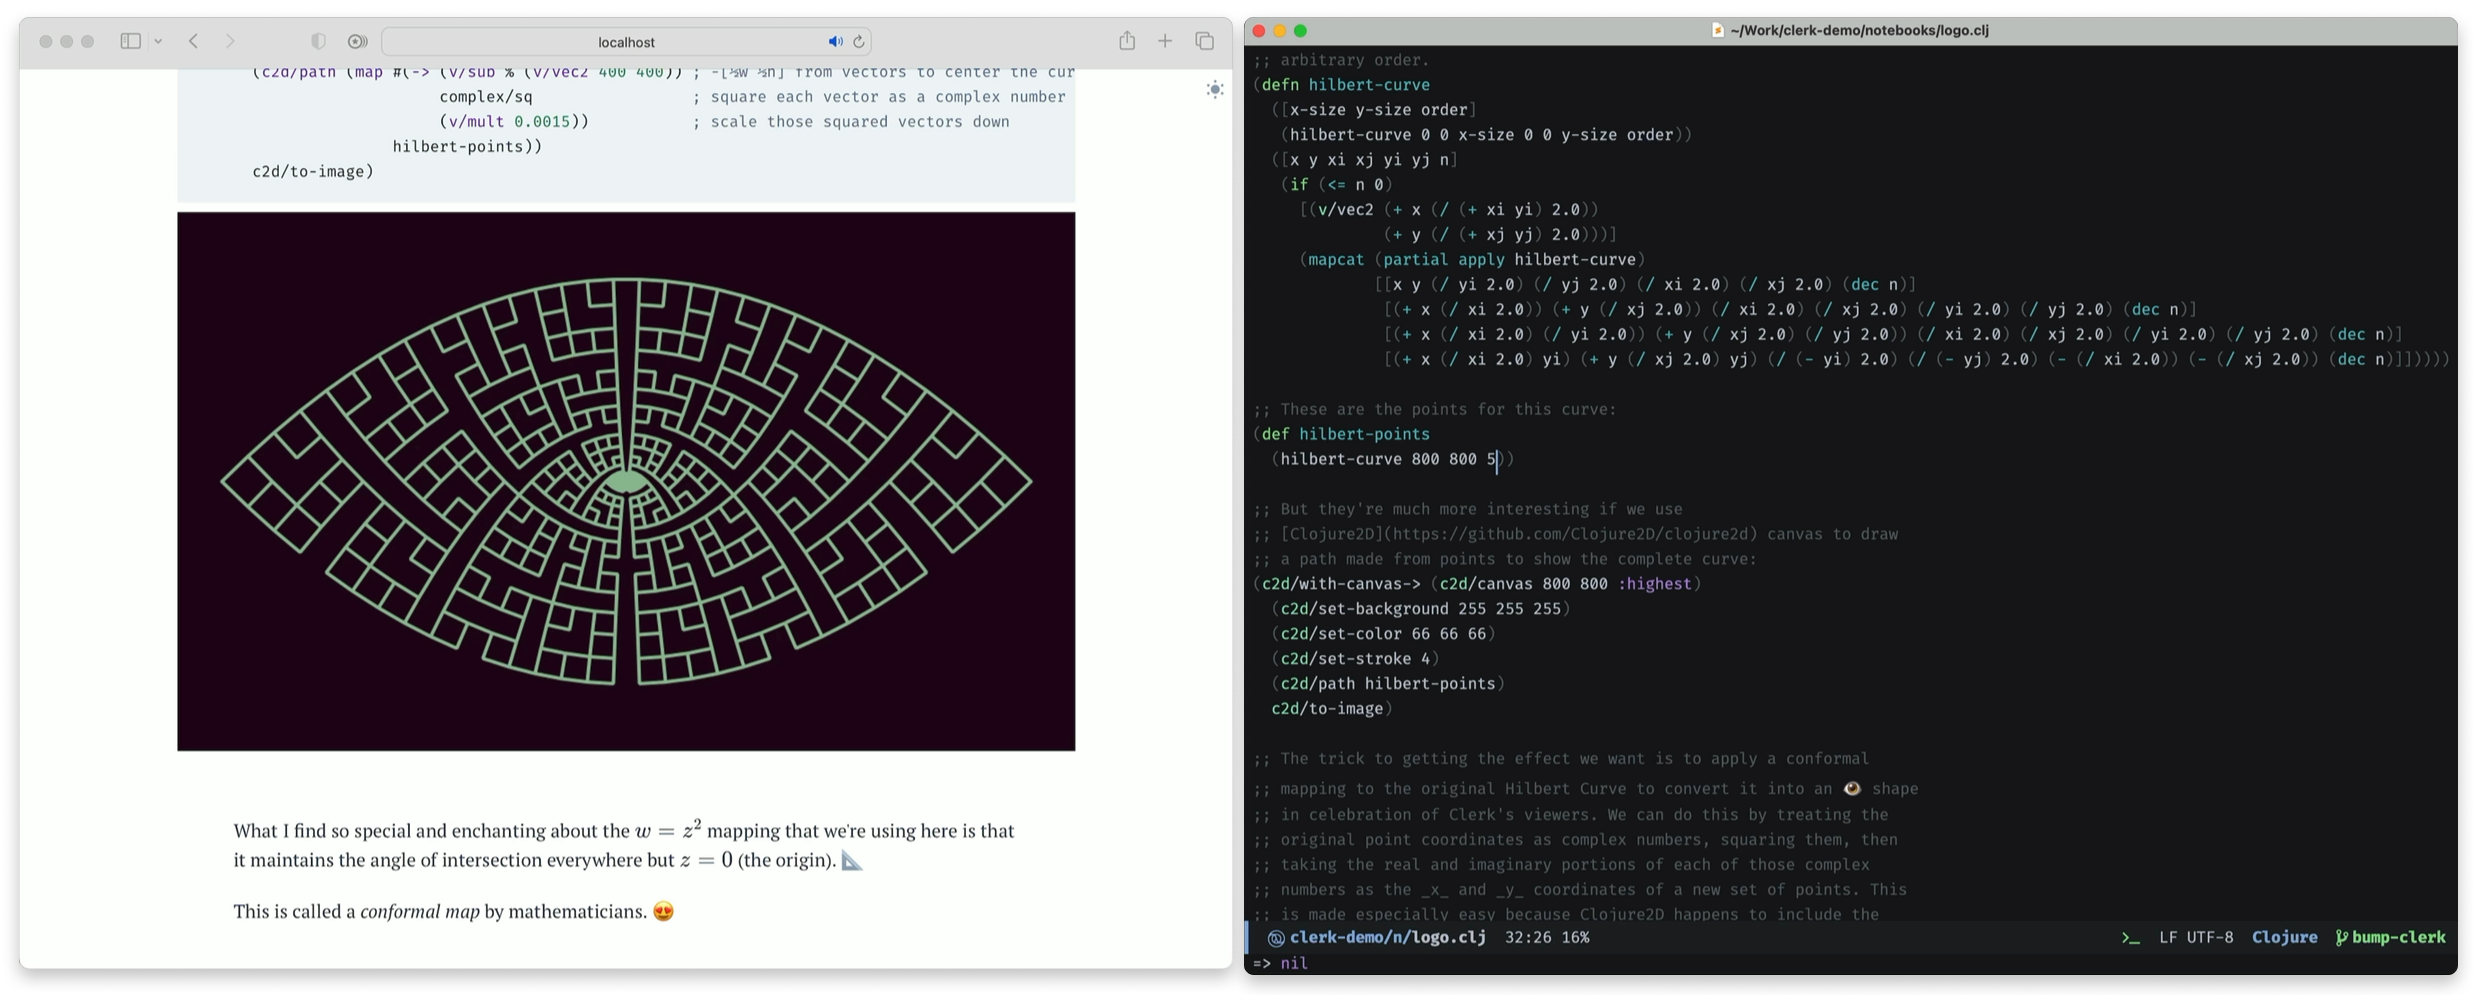
\includegraphics{images/QmSVeZpH3a5ag52AvodLDgBMA3AwnRrfawg5h2SQHk1rY3.png}
\caption{Clerk side-by-side with Emacs}\label{clerk-side-by-side-with-emacs}
}
\end{figure}

As shown here, our \emph{notebooks} are just source files containing regular Clojure code. Block comments are treated as markdown text with added support for LaTeX, data visualization, and so on, while top-level forms are treated as code cells that show the result of their evaluation.\footnote{We have borrowed this approach from {\href{https://maria.cloud}{maria.cloud} (https://maria.cloud)}, a web-hosted interactive Clojure learning tool created by {\href{https://matt.is}{Matt Huebert} (https://matt.is)}, {\href{https://www.daveliepmann.com/}{Dave Liepmann} (https://www.daveliepmann.com/)}, and {\href{https://jackrusher.com/}{Jack Rusher} (https://jackrusher.com/)}. Maria grew out of {\href{https://px16.matt.is}{work presented at PX16} (https://px16.matt.is)} by Matt Huebert.} This format allows us to use Clerk in the context of production code that resides in revision control. Because files decorated with these comment blocks are legal code without Clerk loaded, they can be used in many contexts where traditional notebook-specific code cannot. This has led, among other things, to Clerk being used extensively to publish documentation for libraries that are then able to ship artifacts that have no dependency on Clerk itself.

Clerk's audience is experienced Clojure developers who are familiar with interactive development. They are able to continue programming in their accustomed style, evaluating individual forms and inspecting intermediate results, but with the added ability to \passthrough{\lstinline"show!"} a namespace/file in Clerk. A visual representation of the file is then re-computed either:

\begin{itemize}
\tightlist
\item
  every time the file is saved, using an an optional file watcher; or alternatively,
\item
  via an editor hot-key that can be bound to show the current document. (The authors generally prefer the hot-key over the file watcher, as it feels more direct and gives more control over when to show something in Clerk.)
\end{itemize}

Control and configuration of Clerk primarily occurs through evaluation of Clojure forms from within the programmer\textquotesingle s environment, rather than using outside control panels and settings. This integration with the programmer\textquotesingle s existing tooling eases adoption and allows advanced customization of the system through code.

\hypertarget{fast-feedback:-caching-ux5cux26-incremental-computation}{%
\subsection{Fast Feedback: Caching \& Incremental Computation}\label{fast-feedback:-caching-ux5cux26-incremental-computation}}

To keep feedback loops short, Clerk uses dependency analysis to limit recomputation to forms that haven\textquotesingle t previously been evaluated in Clerk.

In practice this means most changes to a Clerk document are reflected instantly (within 100ms) after saving a file or hitting the keybinding to update the open document.

The caching works on the level of top-level forms. A hash is computed for each top-level form. A change to the form or one of its transitive dependencies will lead to a new hash value.

When Clerk is asked to show a notebook, it will only evaluate forms that aren\textquotesingle t cached in one of Clerk\textquotesingle s two caches:

\begin{itemize}
\tightlist
\item
  an in-memory cache stores a map of the hash of a given form to its current result. This cache is limited to the current forms of the active document.
\item
  An on-disk-cache stores the same information but to allow the user to continue work after a restart without recomputing potentially expensive operations.\footnote{In tasks with intensive data preparation steps, this savings can be considerable.} Because Clojure supports lazy evaluation of potentially infinite sequences, safeguards are in place to skip caching unreasonable values.
\end{itemize}

This caching behavior can be fine-tuned (or disabled) down to the level of individual forms.

The on-disk caches use a content-addressed store where each result is stored using a filename derived from the SHA-2 hash of its contents. We use the self-describing {\href{https://multiformats.io/multihash/}{multihash format}\footnote{https://multiformats.io/multihash/}} which combines an identifier of the hash function with its digest length and value to support future changes of the hash algorithm. Additionally, a file named after the hash of a form contains a pointer to its results filename.

This combination of immutability and indirection makes distributing the cache trivial using last-write wins for the tiny (90 bytes) pointer files. The content-addressed result cache files are never changed and can thus be synchronized without conflict.

\begin{quote}
While I did believe, and it has been true in practice, that the vast majority of an application could be functional, I also recognized that almost all programs would need some state. Even though the host interop would provide access to (plenty of) mutable state constructs, I didn't want state management to be the province of interop; after all, a point of Clojure was to encourage people to stop doing mutable, stateful OO. In particular I wanted a state solution that was much simpler than the inherently complex locks and mutexes approaches of the hosts for concurrency-safe state. And I wanted something that took advantage of the fact that Clojure programmers would be programming primarily with efficiently persistent immutable data. \cite{Hickey_2020}

-- Rich Hickey
\end{quote}

It is idiomatic in Clojure to use boxed containers to manage mutable state.\footnote{{\href{https://clojure.org/about/state}{Values and Change: Clojure's approach to Identity and State} (https://clojure.org/about/state)}} While there are several of these constructs in the language, in practice {\href{https://clojure.org/reference/atoms}{atoms}\footnote{https://clojure.org/reference/atoms}} are the most popular by far. An atom allows reading the current value inside it with {\href{https://clojuredocs.org/clojure.core/deref}{\passthrough{\lstinline!deref/@!}}} and updating it\textquotesingle s value with {\href{https://clojuredocs.org/clojure.core/swap!}{\passthrough{\lstinline"swap!"}}}.

When Clerk encounters an expression in which an atom\textquotesingle s mutable value is being read using \passthrough{\lstinline!deref!}, it will try to compute a hash based on the value \emph{inside} the atom  at runtime, and extend the expression\textquotesingle s static hash with it.

This extension makes Clerk\textquotesingle s caching work naturally with idiomatic use of mutable state, and frees programmers from the need to manually opt out of caching for those expressions.

\hypertarget{semantic-differences-from-regular-clojure}{%
\subsection{Semantic Differences from Regular Clojure}\label{semantic-differences-from-regular-clojure}}

Clojure uses a single-pass, whole-file compilation strategy in which each evaluated form is added to the state of the running system. One positive aspect of this approach is that manually evaluating a series of forms produces the same result as loading a file containing the same forms in the same order, which is a useful property when interactively building up a program.

A practical concern with this sort of ``bottom-up" programming is that the state of the system can diverge from the state of the source file, as forms that have been deleted from the source file may still be present in the running system. This can lead to a situation where newly written code depends on values that will not exist the next time the program runs, causing surprising errors. To help avoid this, Clerk defaults to signaling an error unless it can resolve all referenced definitions in the runtime to the source code.

It is our goal to match the semantics of Clojure as closely as possible but as a very dynamic language, there are limits to what Clerk\textquotesingle s analysis can handle. Here are some of the things we currently do not support:

\begin{itemize}
\tightlist
\item
  Multiple definitions of the same var in a file
\item
  Setting dynamic variables using {\href{https://clojuredocs.org/clojure.core/set!}{\passthrough{\lstinline"set!"}}}
\item
  Dynamically altering vars using {\href{https://clojuredocs.org/clojure.core/alter-var-root}{\passthrough{\lstinline!alter-var-root!}}}
\item
  Temporarily redefining vars using {\href{https://clojuredocs.org/clojure.core/with-redefs}{\passthrough{\lstinline!with-redefs!}}}
\end{itemize}

We have included a mechanism to override Clerk\textquotesingle s error checking in cases where the user knows that one or more of these techniques are in use.

\hypertarget{presentation}{%
\subsection{Presentation}\label{presentation}}

Clerk uses a client/server architecture. The server runs in the JVM process that hosts the user\textquotesingle s development environment. The client executes in a web browser running an embedded Clojure interpreter.\footnote{{\href{https://github.com/babashka/sci}{Small Clojure Interpreter} (https://github.com/babashka/sci)} by Michiel Borkent}

The process of conveying a value to the client is a \emph{presentation}, a
term taken from Common Lisp systems that support similar features.\footnote{This feature originated on the Lisp Machine, and lives on in a reduced form as a feature of the emacs package {\href{https://slime.common-lisp.dev/doc/html/Presentations.html}{Slime} (https://slime.common-lisp.dev/doc/html/Presentations.html)}.} The process of presentation makes use of \emph{viewers}, each of which is a hash map from well-known keys to quoted forms containing source code for Clojure functions that specify how the client should render data structures of a given type. When a viewer form is received on the client side, it is compiled into a function that will be then called on data later sent by the server.

When the \passthrough{\lstinline!present!} function is called on the server side, it defaults to performing a depth-first traversal of the data structure it receives, attaching appropriate viewers at each node of the tree. The resulting structure containing both data and viewers is then sent to the client.

To avoid overloading the browser or producing uselessly large output, Clerk's built-in collection viewer carries an attribute to control the number of items initially displayed, allowing more data to be requested by the user on demand. Besides this simple limit, there's a second global \emph{budget} per result to limit the total number of items shown in deeply nested data structures. We've found this simple system to work fairly well in practice.

One benefit of using the browser for Clerk\textquotesingle s rendering layer is that it can produce static HTML pages for publication to the web. We could not resist the temptation to produce this document with Clerk.

It\textquotesingle s also possible to use Clerk\textquotesingle s presentation system in other contexts. We know of at least one case of a user leveraging Clerk\textquotesingle s presentation system to do in-process rendering without a browser.\footnote{See {\href{https://github.com/phronmophobic/desk}{Desk} (https://github.com/phronmophobic/desk)}, by Adrian Smith.}

\hypertarget{built-in-viewers}{%
\subsection{Built-in Viewers}\label{built-in-viewers}}

Clerk comes with a set of built-in viewers for common situations. These include support for Clojure's immutable data structures, HTML (including the {\href{https://github.com/weavejester/hiccup}{hiccup variant}\footnote{https://github.com/weavejester/hiccup}} that is often used in Clojure to represent HTML and SVG), data visualization, tables, LaTeX, source code, images, and grids, as well as a fallback viewer based on Clojure's printer. The {\href{https://book.clerk.vision}{Book of Clerk}\footnote{https://book.clerk.vision}} gives a good overview of the available built-ins. Because Clerk's client is running in the browser, we are able to benefit from the vast JS library ecosystem. For example we\textquotesingle re using {\href{https://plotly.com/javascript/}{Plotly}\footnote{https://plotly.com/javascript/}} and {\href{https://github.com/vega/vega-embed}{vega}\footnote{https://github.com/vega/vega-embed}} for graphing, {\href{https://codemirror.net}{CodeMirror}\footnote{https://codemirror.net}} for rendering code cells, and {\href{https://katex.org}{KaTeX}\footnote{https://katex.org}} for typesetting mathematics.

Clerk's built-in viewers try to suit themselves to typical Data Science use cases. By default, Clerk shows a code block's result as-is with some added affordances like syntax coloring and expandability of large sub-structures that are collapsed by default.

Here is an interactive example of the well-known \passthrough{\lstinline!iris!} data set, which we\textquotesingle ve added as a dependency to this notebook. Clicking the disclosure triangles will expand the data structure:

\begin{minipage}{\linewidth}
\begin{lstlisting}
datasets/iris
\end{lstlisting}
\end{minipage}


\includegraphics{images/anon-expr-5dtc44qrw3zUvpTfiAXJDH7mtADdRT-result.png}

Additional affordances are automatic expansion of a nested data structure based on its shape and expanding multiple sub-structures on the same level, as demonstrated in this video:

\begin{figure}
\hypertarget{expanding-multiple-sub-structures-at-once}{%
\centering
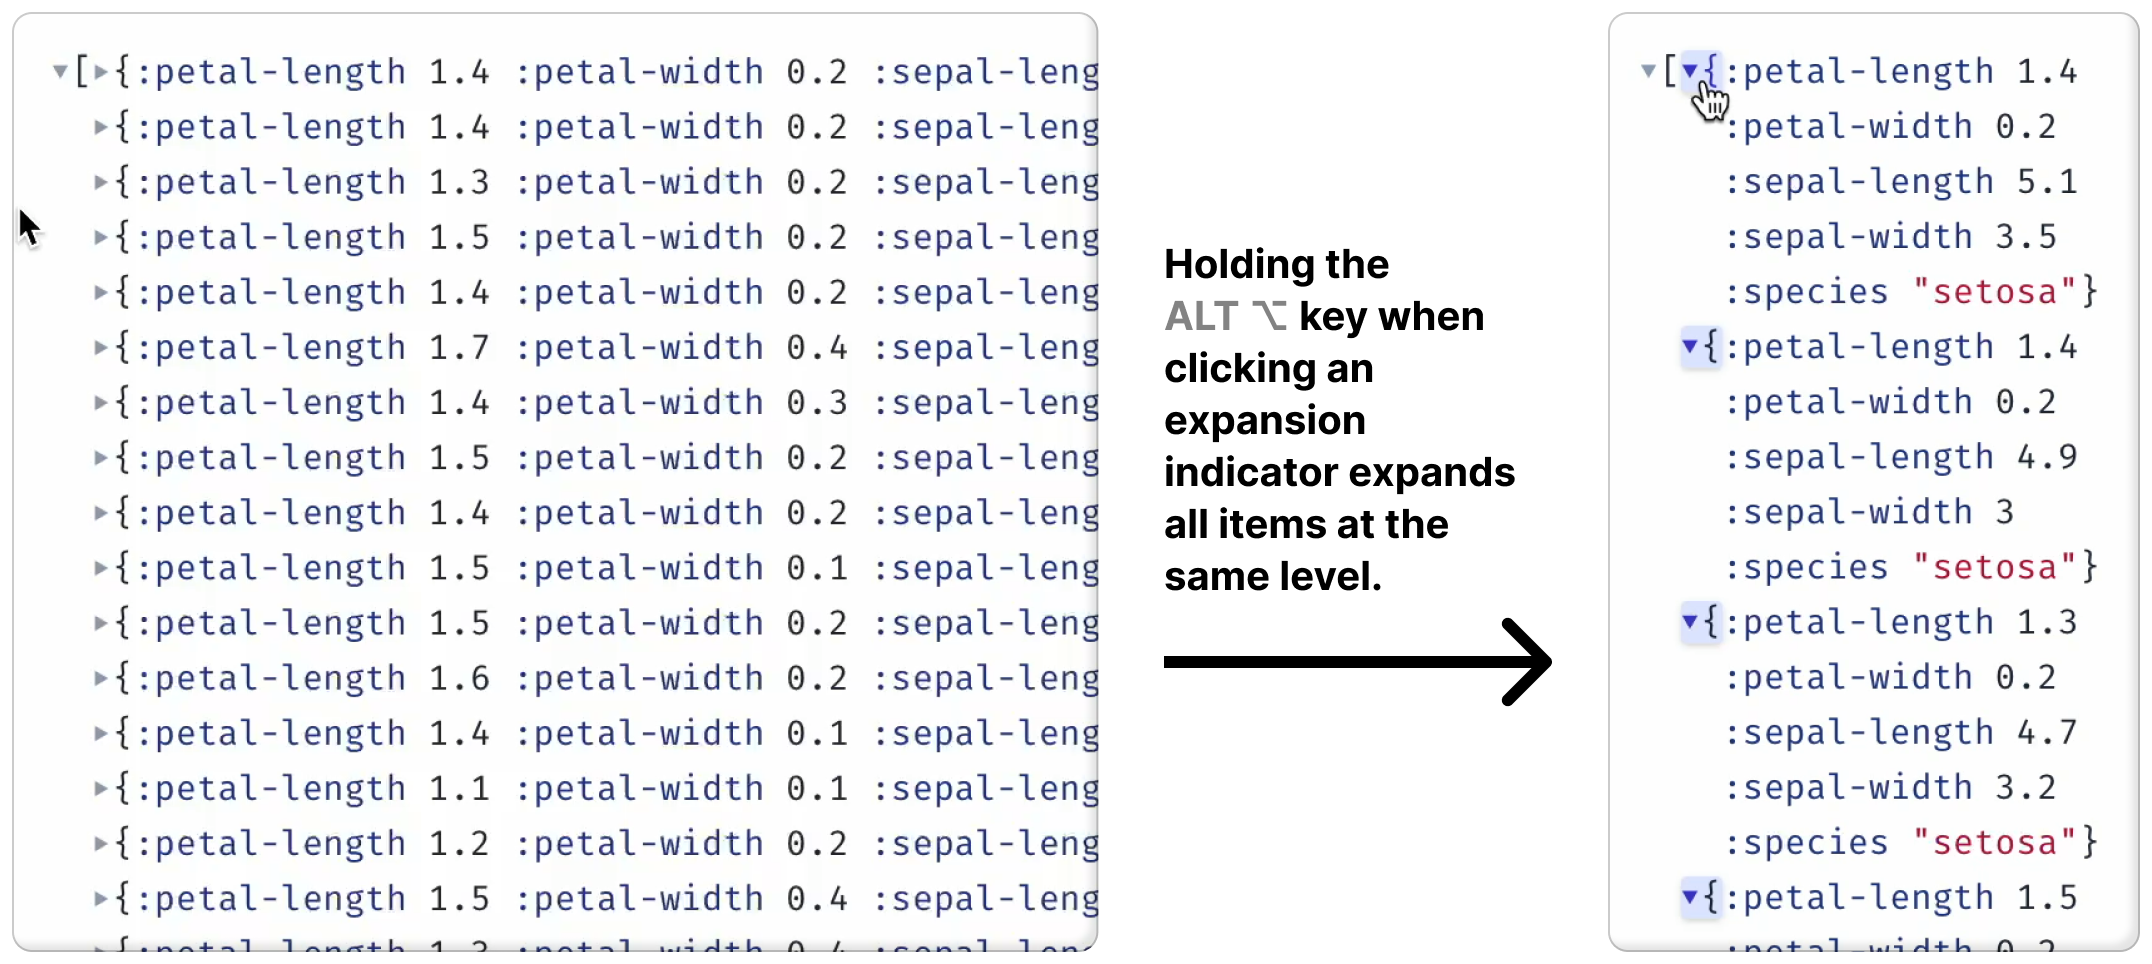
\includegraphics{images/QmcABdFREVjdAcruW3Qb45PLAwD7E337BWgU2gvU2gXw1B.png}
\caption{Expanding multiple sub-structures at once}\label{expanding-multiple-sub-structures-at-once}
}
\end{figure}

Using the built-in \passthrough{\lstinline!clerk/table!} viewer, the same data structure can also be rendered as a table. The table viewer uses heuristics to infer the makeup of the table, such as column headers, from the structure of the data:
\vspace{2em}

\begin{minipage}{\linewidth}
\begin{lstlisting}
(clerk/table datasets/iris)
\end{lstlisting}
\end{minipage}

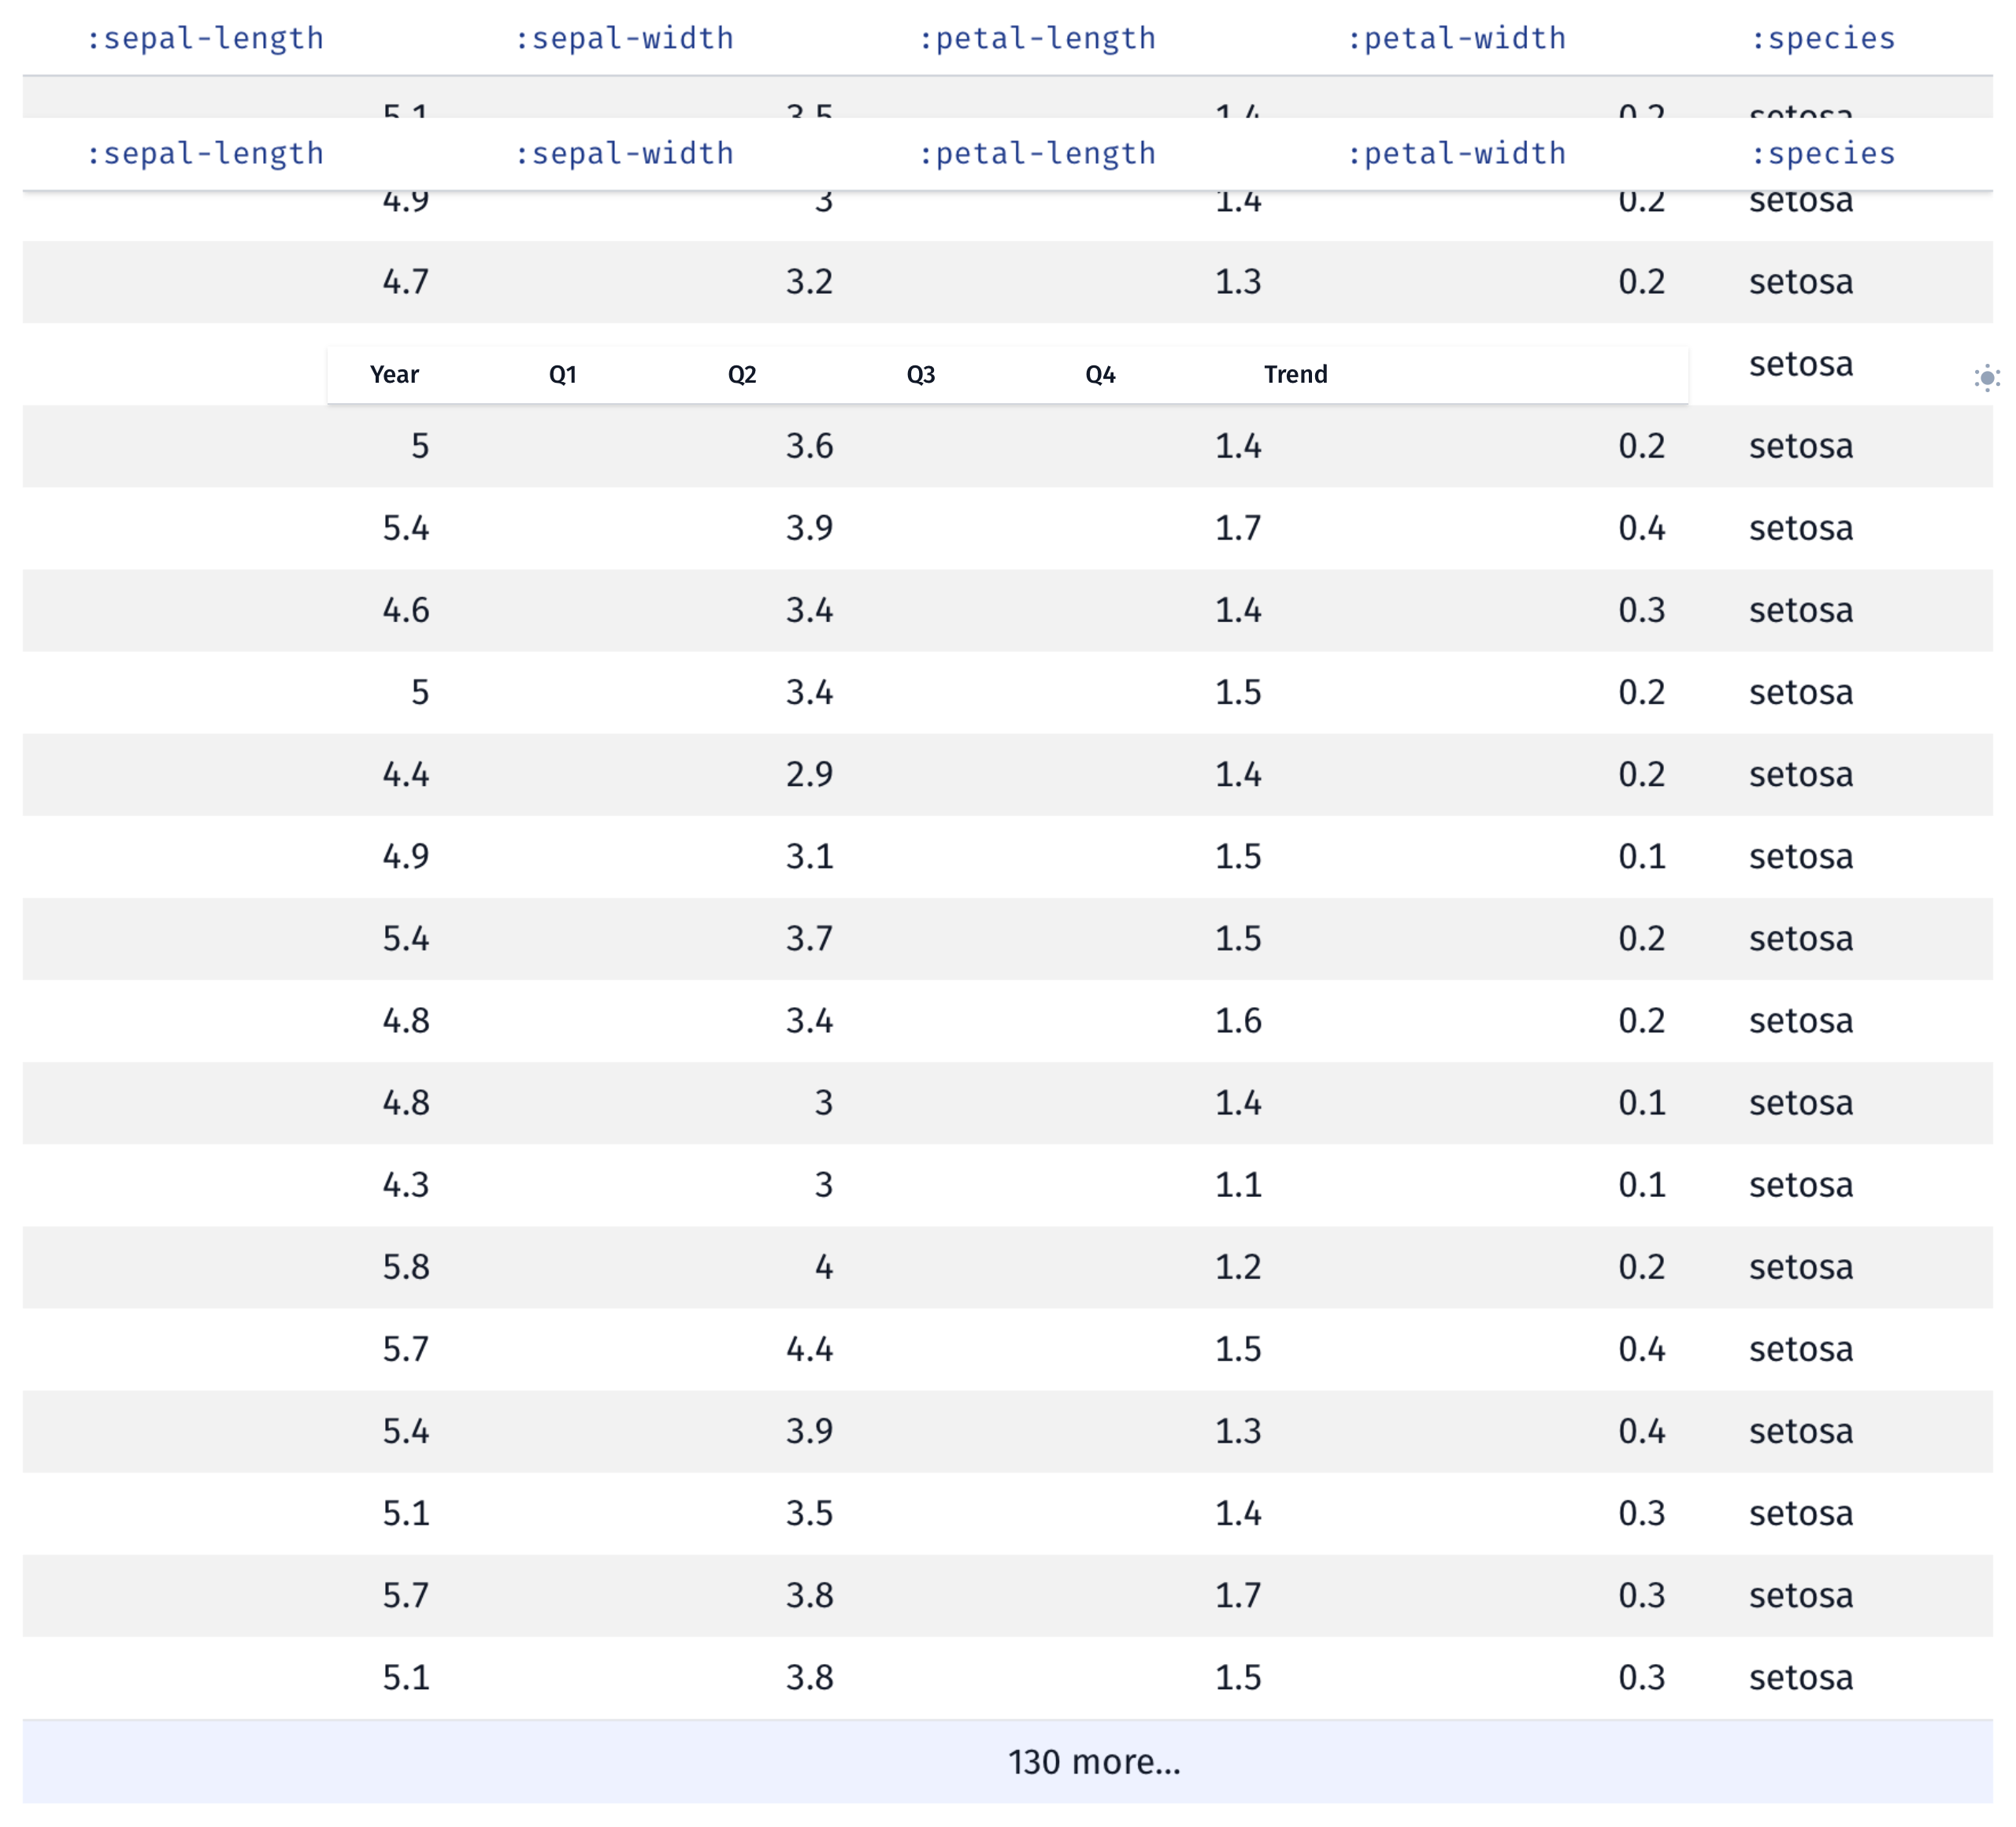
\includegraphics[width=0.45\textwidth]{images/anon-expr-5dtuc4aWdsThsN1ZehoANzcdjAoyh5-result.png}

\vspace{4em}
Together with tables, plots are the most commonly used viewer for Data Science use cases. In the following figure, the same \passthrough{\lstinline!iris!} dataset, as shown in the above table example, is used to render an interactive {\href{https://vega.github.io/vega-lite/}{Vega-Lite}\footnote{https://vega.github.io/vega-lite/}} plot using the \passthrough{\lstinline!clerk/vl!} viewer:
\vspace{2em}

\begin{minipage}{\linewidth}
\begin{lstlisting}
(clerk/vl {:data {:values datasets/iris}
           :width 500
           :height 500
           :title "sepal-length vs. sepal-width"
           :mark {:type "point"
                  :tooltip {:field :species}}
           :encoding {:color {:field :species}
                      :x {:field :sepal-length
                          :type :quantitative
                          :scale {:zero false}}
                      :y {:field :sepal-width
                          :type :quantitative
                          :scale {:zero false}}}
           :embed/opts {:actions false}})
\end{lstlisting}
\end{minipage}

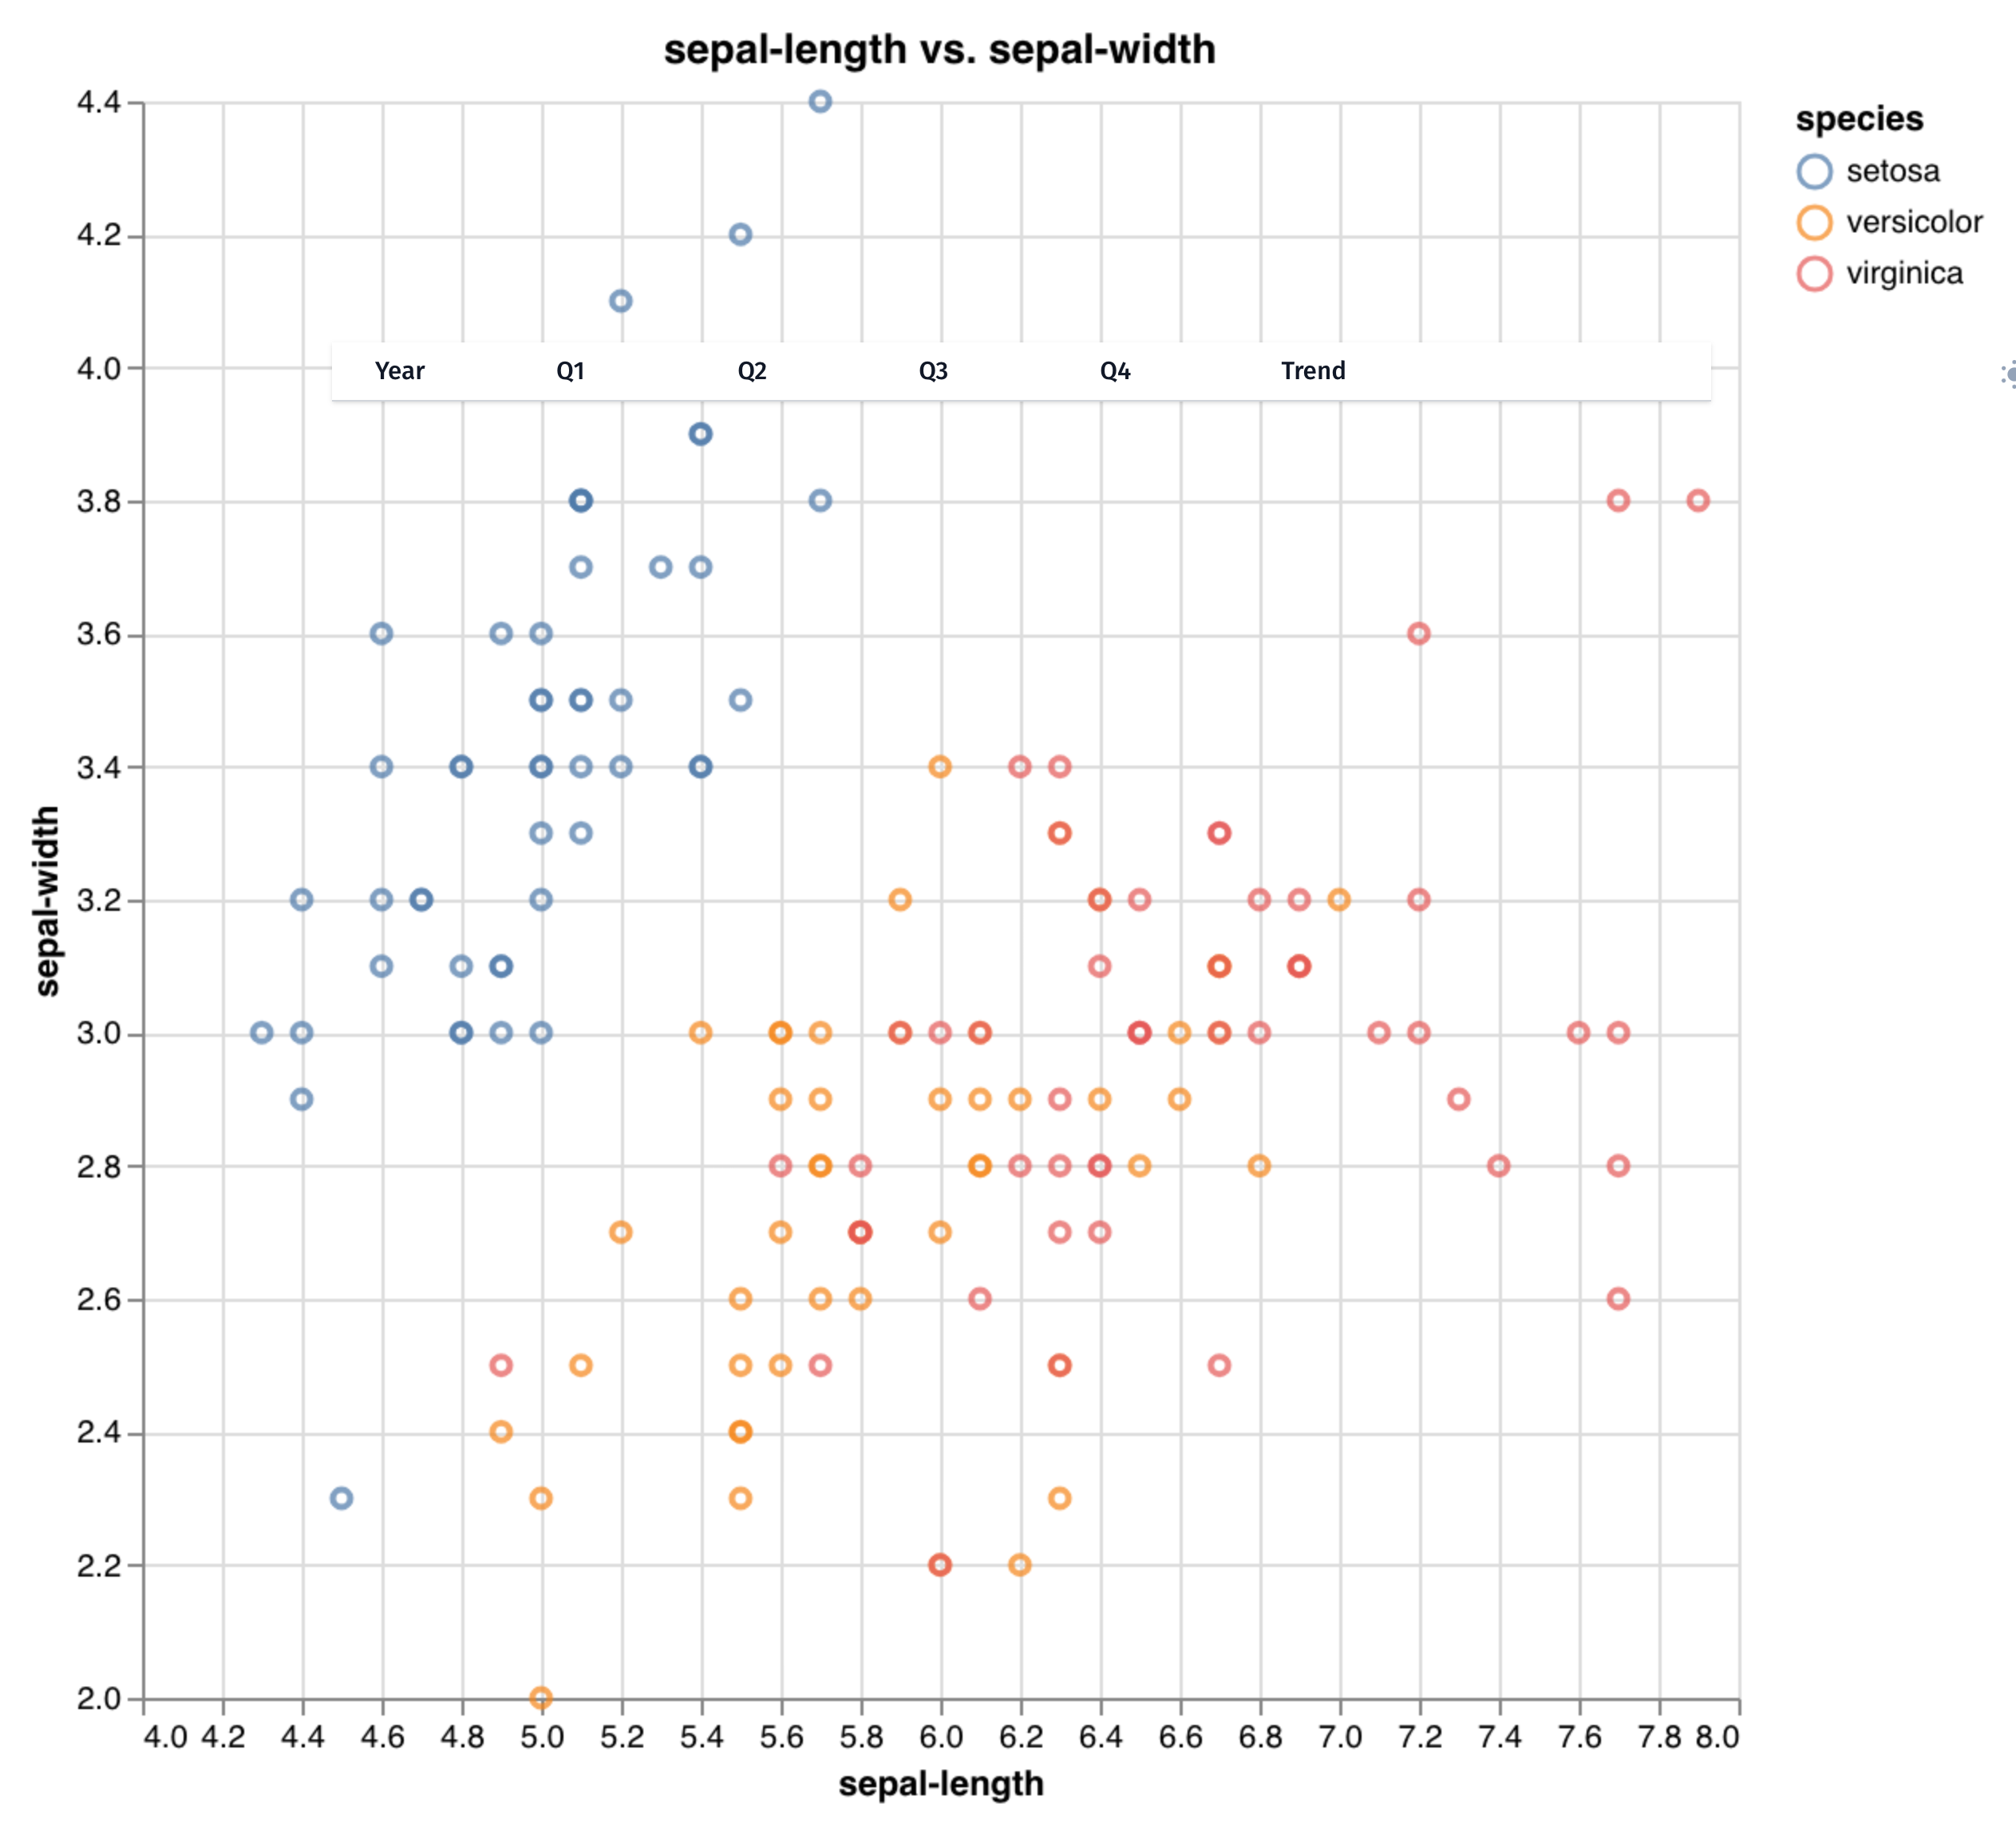
\includegraphics{images/anon-expr-5dtjeGHWCqJb9X8RfQtspB6Cyeo8Yv-result.png}

It is important to note that Clerk's viewers work in a way that encourages composition. Multiple viewers can be combined to suit a specific use case such as the following example showing a table of airline passenger numbers\footnote{using a {\href{https://github.com/applied-science/edn-datasets}{Clojure port} (https://github.com/applied-science/edn-datasets)} of R's built-in dataset of {\href{https://search.r-project.org/R/refmans/datasets/html/AirPassengers.html}{Box \& Jenkins classic airline data} (https://search.r-project.org/R/refmans/datasets/html/AirPassengers.html)}.} by year and quarter and embedding a sparkline graph into the table row for each year.

A typical Clerk workflow for this would be to first take a look at the shape of the data:

\begin{minipage}{\linewidth}
\begin{lstlisting}
datasets/air-passengers
\end{lstlisting}
\end{minipage}


\includegraphics{images/anon-expr-5drcDeJRcpX2uPqZi7XJch2DedHM6j-result.png}

Then, a \passthrough{\lstinline!sparkline!} function is defined and tested to generate graphs (using \passthrough{\lstinline!clerk/vl!}) that will be embedded into each table row later:

\begin{minipage}{\linewidth}
\begin{lstlisting}
(defn sparkline [values]
  (clerk/vl {:data {:values (map-indexed (fn [i n] {:x i :y n}) values)}
             :mark {:type :line :strokeWidth 1.2}
             :width 140
             :height 20
             :config {:background nil :border nil :view {:stroke "transparent"}}
             :encoding {:x {:field :x :type :ordinal :axis nil :background nil}
                        :y {:field :y :type :quantitative :axis nil :background nil}}
             :embed/opts {:actions false}}))
\end{lstlisting}
\end{minipage}


\includegraphics{images/sparkline-result.png}

\begin{minipage}{\linewidth}
\begin{lstlisting}
(sparkline (shuffle (range 30)))
\end{lstlisting}
\end{minipage}


\includegraphics[width=0.15\textwidth]{images/anon-expr-5dr3uWTA777Ny4ajSWGaWCymacQXhQ-result.png}

Finally, the data is reduced to quarters and years, adding the sparkline graphs in a final step:

\begin{minipage}{\linewidth}
\begin{lstlisting}
(clerk/table
 {:head ["Year" "Q1" "Q2" "Q3" "Q4" "Trend"]
  :rows (->> datasets/air-passengers
             (group-by :year)
             (map (fn [[year months]]
                    (let [qs (->> months (map :n)
                                  (partition 3)
                                  (map #(reduce + %)))]
                      (concat [year]
                              qs
                              [(sparkline
                                (map :n months))]))))
             (sort-by first))})
\end{lstlisting}
\end{minipage}

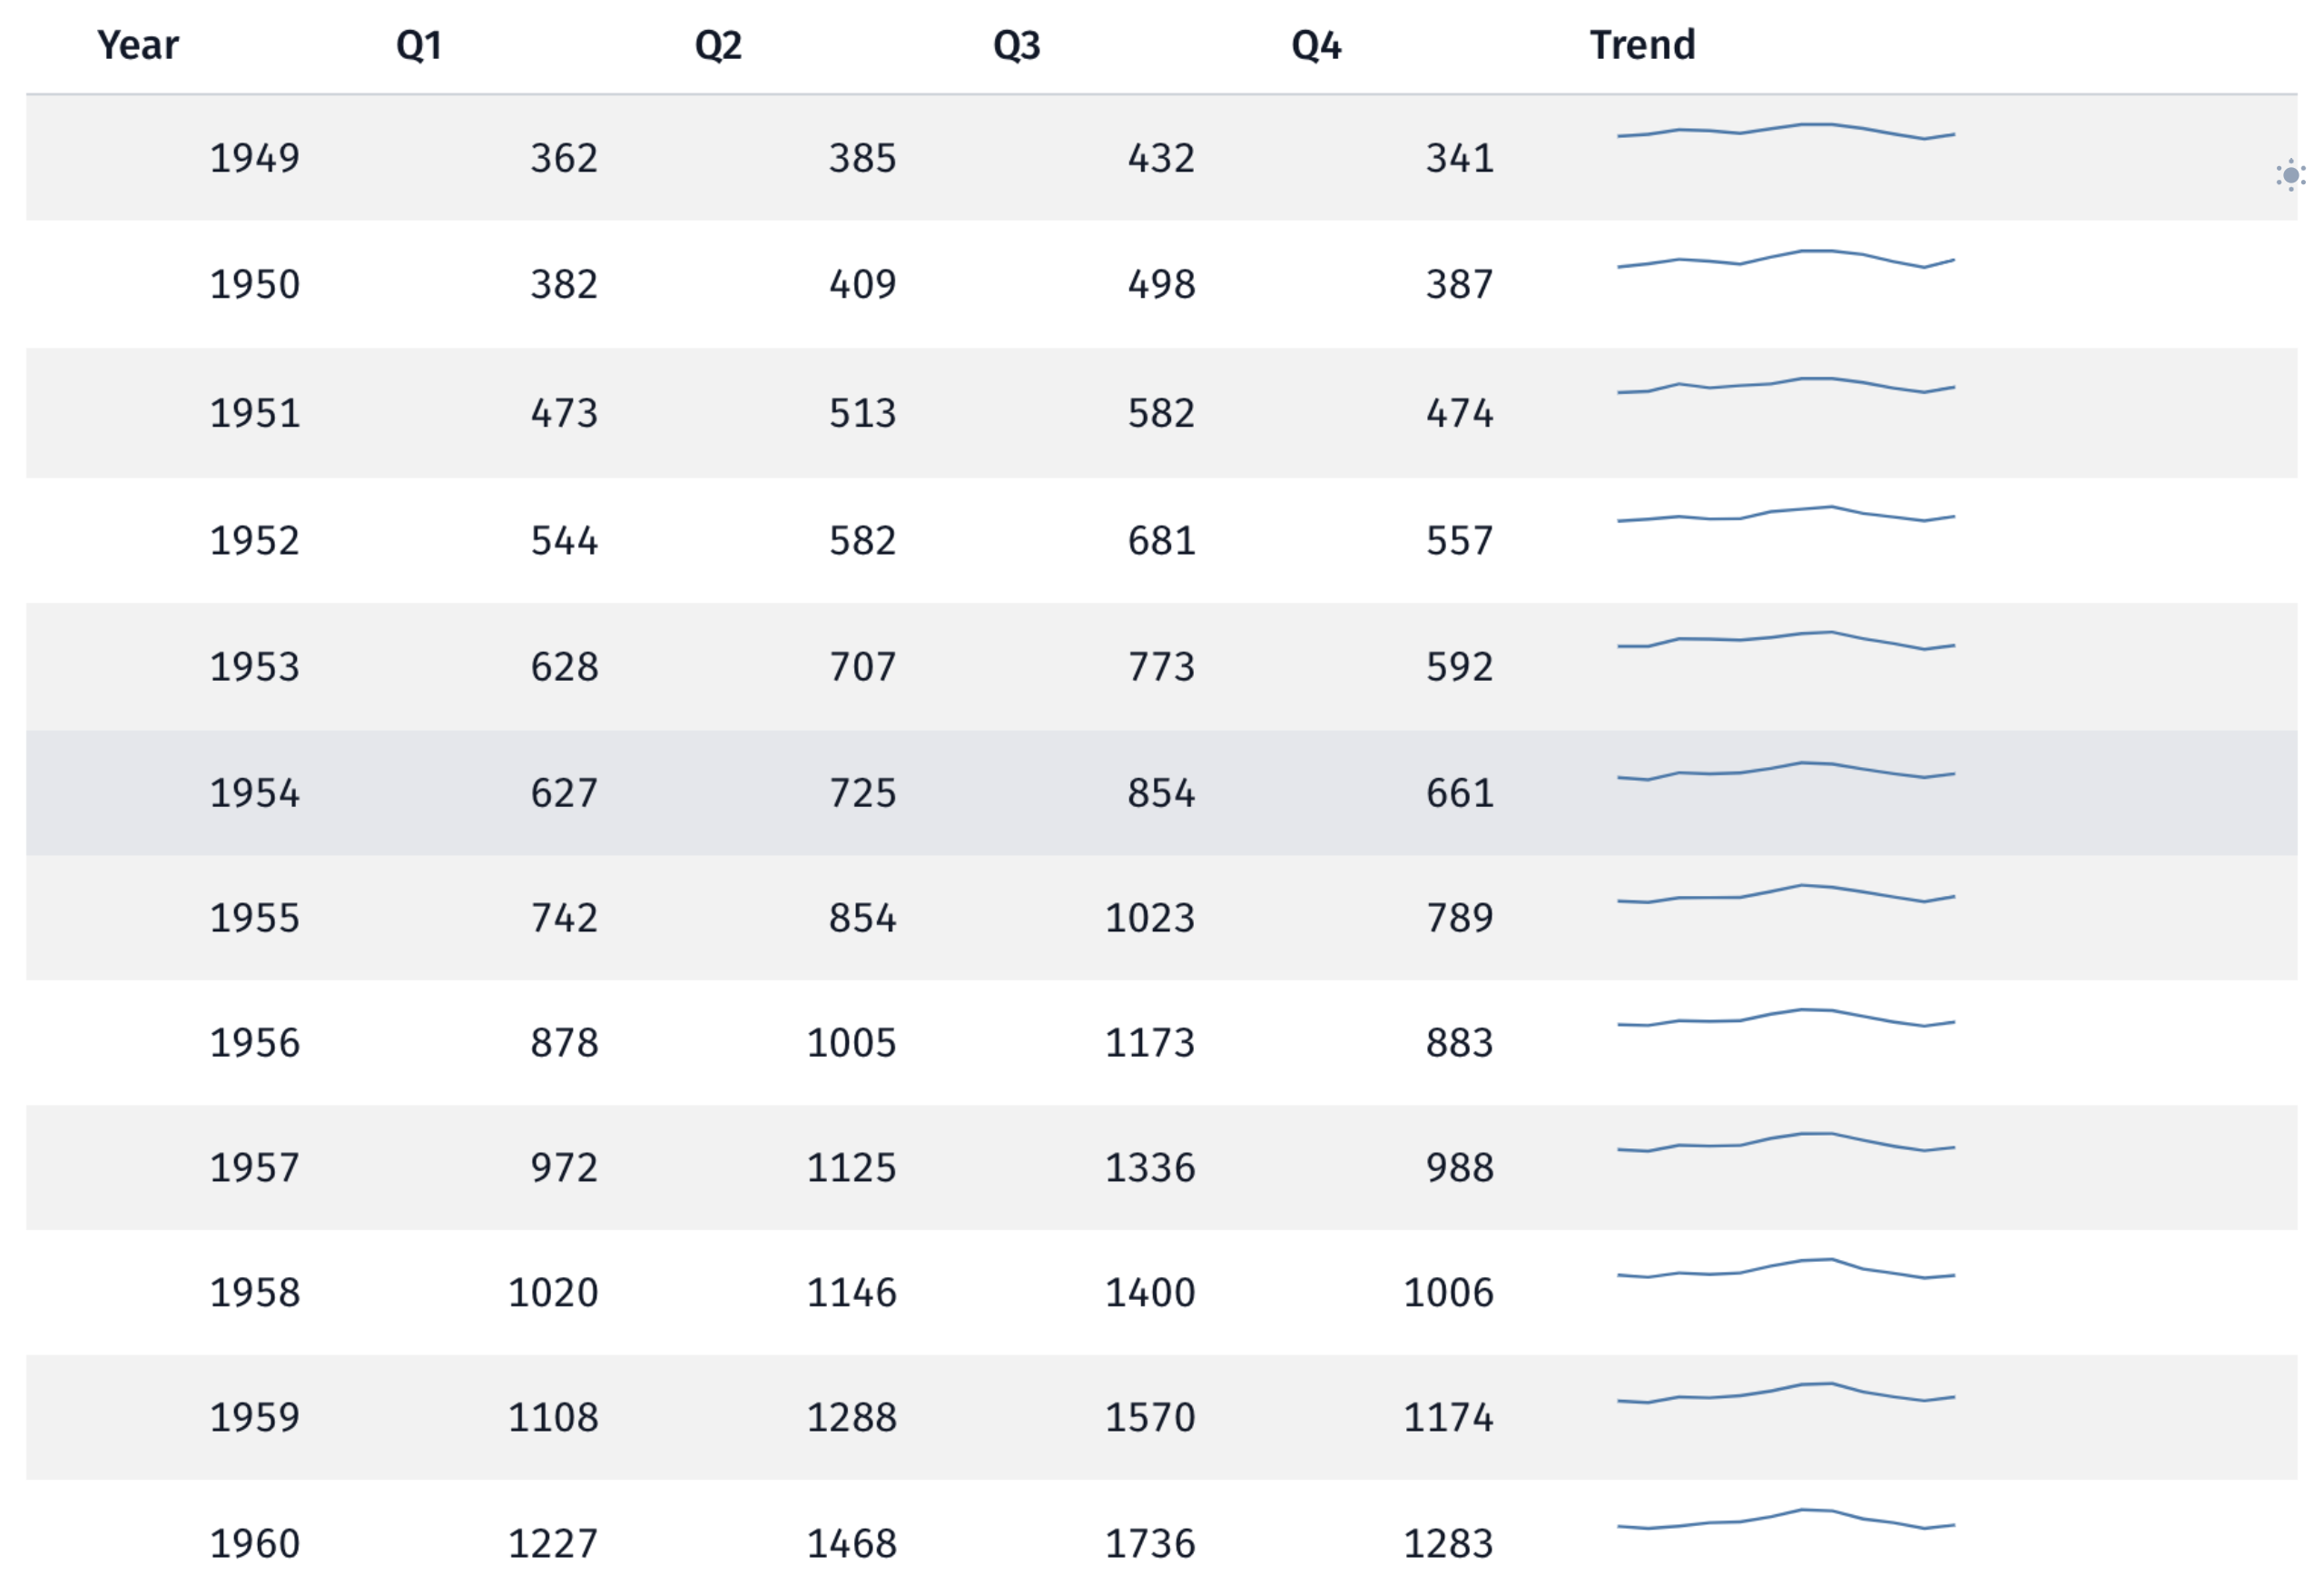
\includegraphics[width=0.45\textwidth]{images/anon-expr-5dr28YWkT1KitTsVou6NEy6JRWh9wg-result.png}

This sort of gradual refinement is a hallmark of exploratory programming, and is especially enjoyable with access to the full power of a general purpose programming language.

\hypertarget{moldable-viewer-api}{%
\subsection{Moldable Viewer API}\label{moldable-viewer-api}}

Clerk's viewers are an ordered (and thus prioritized) collection of plain Clojure hash maps. Clerk interprets the following optional keys in each viewer map:

\begin{itemize}
\tightlist
\item
  \passthrough{\lstinline!:pred!} is a predicate function that tests whether this viewer should be used for a given data structure
\item
  \passthrough{\lstinline!:transform-fn!} is an optional function run on the server side to transform data before sending it to the client. It receives a map argument with the original value under a key. Additional keys carry the path, the viewer stack, and the budget (for elision)
\item
  \passthrough{\lstinline!:render-fn!} is a quoted form that will be sent to the browser, where it will be turned into a function that will be called to display the data
\item
  \passthrough{\lstinline!:page-size!} is a number that indicates how many items to send in each chunk during elision/pagination
\end{itemize}

Here, for example, is the \passthrough{\lstinline!code!} viewer, which shows a piece of Clojure code with idiomatic syntax highlighting:\footnote{The source code here is rendered by the viewer that it describes.}

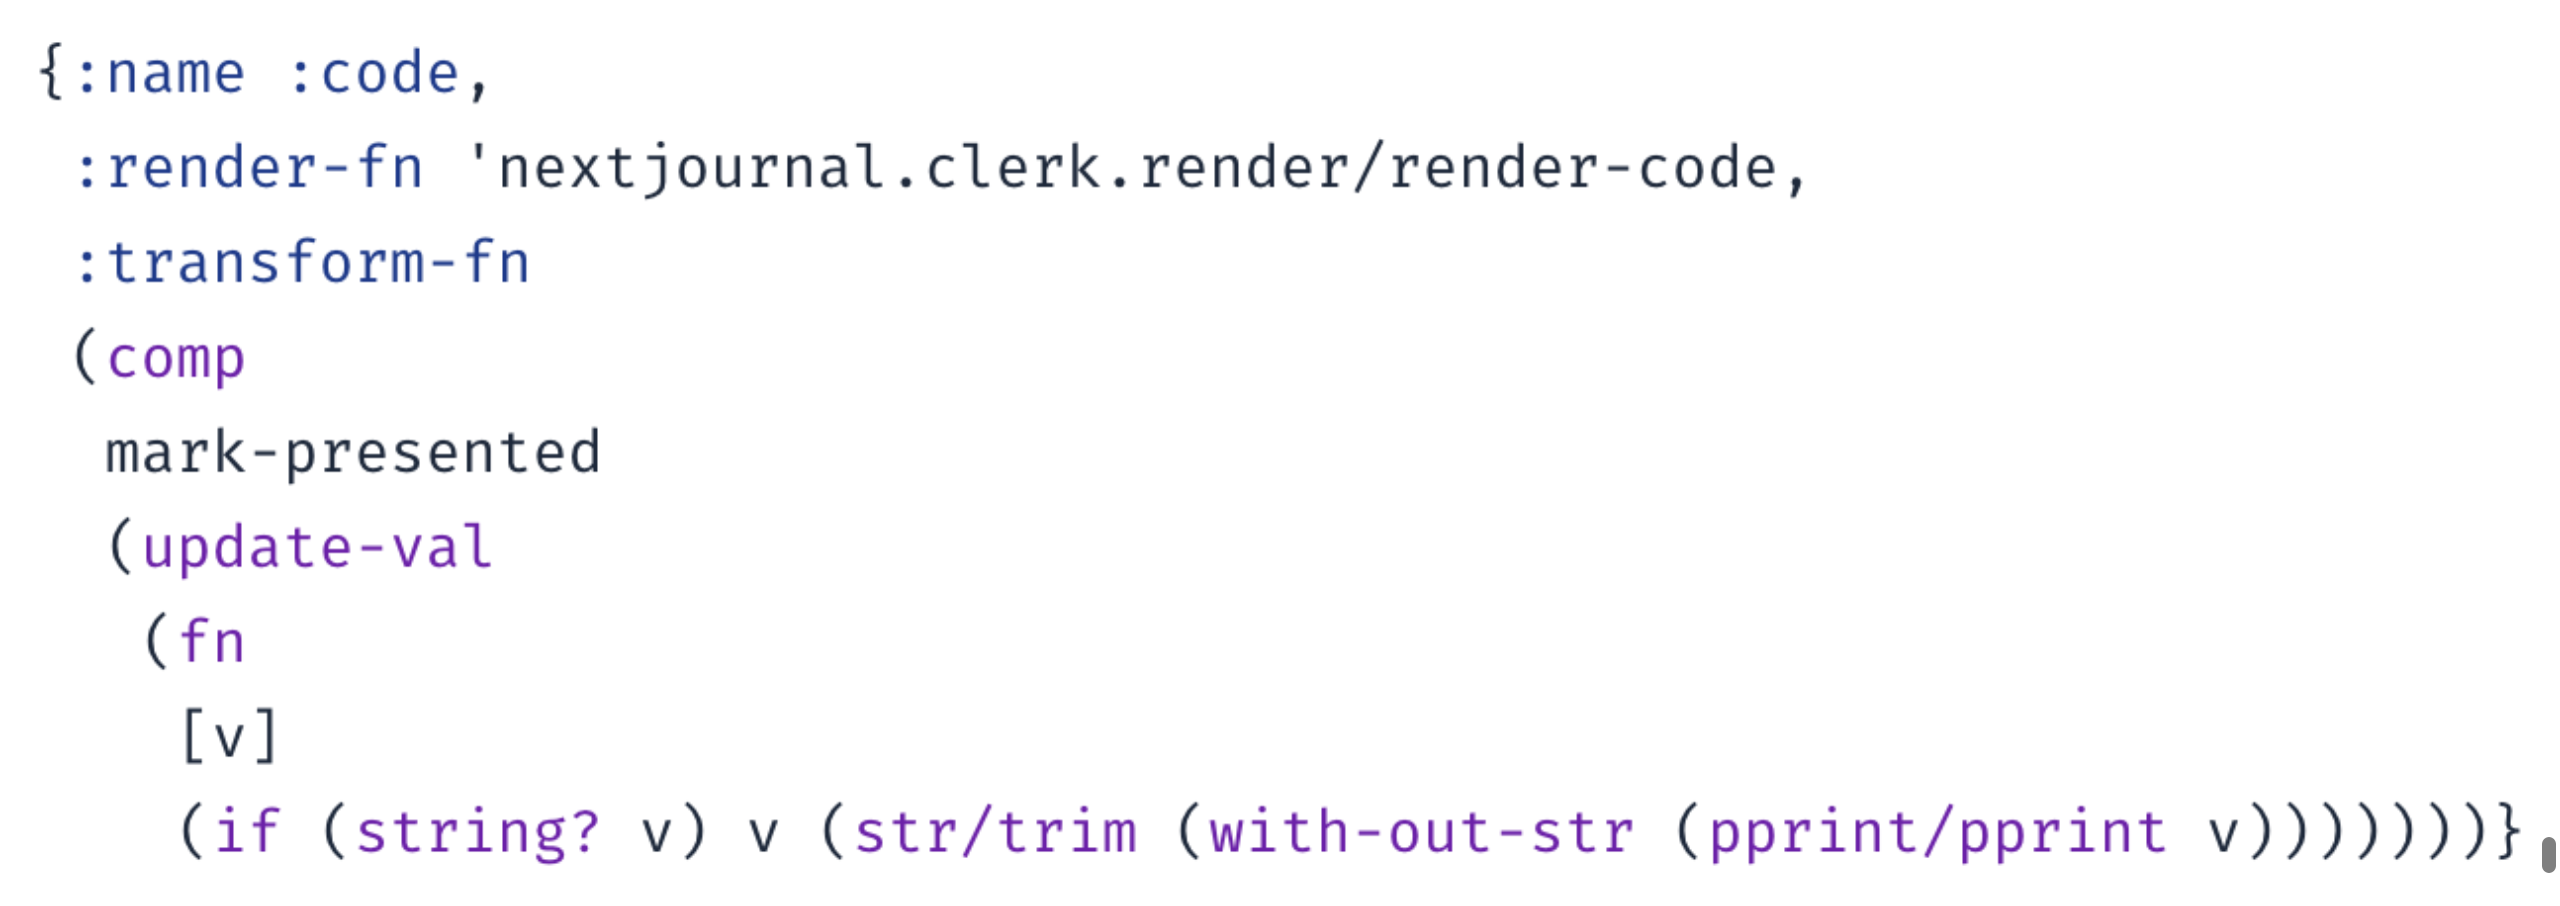
\includegraphics{images/anon-expr-5drCPuwp8LirNTWeyr5WSDHWVV2rnC-result.png}

Viewers can also be explicitly selected by wrapping a value in the \passthrough{\lstinline!clerk/with-viewer!} function, which produces a presentation for that value using that viewer. Alternatively, viewers can be selected by placing a Clojure metadata declaration before a form. Because of the way Clojure handles compilation, metadata in this position is ultimately ignored in the generated code. So far as we know, this is a novel mechanism for out-of-band signaling to a specialized Clojure parser.

The process of selecting viewers happens programmatically on the server side, thus using the programmer\textquotesingle s already existing interactive programming environment as a user interface.

\hypertarget{sync}{%
\subsection{Sync}\label{sync}}

To help with creating interactive tools using Clerk, it also supports bidirectional sync of state between the client and server Clojure environments. If a Clojure \passthrough{\lstinline!atom!} on the server is annotated with metadata indicating it is \passthrough{\lstinline!sync!}, Clerk will create a corresponding var in the client environment. Both of these atoms will be automatically instrumented with an update watcher that broadcasts a \emph{diff} to the other side.

In addition, a server-side change will trigger a refresh of the currently active document, which will then re-calculate the minimum subset of the document that is dependent on that atom\textquotesingle s value. This allows us to use Clerk for small local-first apps, as shown in \autoref{interactive-regex-dictionary}.

\hypertarget{tap-stream-inspector}{%
\subsection{Tap Stream Inspector}\label{tap-stream-inspector}}

Clerk also comes with an inspector for Clojure\textquotesingle s tap system.

\begin{quote}
\textbf{tap} is a shared, globally accessible system for distributing a series of informational or diagnostic values to a set of (presumably effectful) handler functions. It can be used as a better debug prn, or for facilities like logging etc.

-- {\href{https://github.com/clojure/clojure/blob/0b42eab4bfca5270e0d2b2e58d83b1e2c8a85473/changes.md\#23-tap}{Clojure 1.10 Changelog}}
\end{quote}

When enabled, Clerk will attach a tap listener function and record and show the tap stream. This makes Clerk\textquotesingle s viewer system accessible across file and namespace boundaries and independently of the caching mechanisms.

\hypertarget{embedding-examples}{%
\subsection{Embedding Examples}\label{embedding-examples}}

The {\href{https://clojuredocs.org/clojure.core/comment}{comment}} macro in Clojure is typically used to annotate source code with rich examples that exercise the program during development and aid comprehension.

Clerk\textquotesingle s example macro expands on that by showing the source code next to the evaluation result.

\begin{minipage}{\linewidth}
\begin{lstlisting}
(clerk/example
  (+ 40 2)
  (-> 42 range shuffle)
  (clerk/code (macroexpand '(clerk/example (inc 41))))
  (clerk/html [:h1 "👋"]))
\end{lstlisting}
\end{minipage}

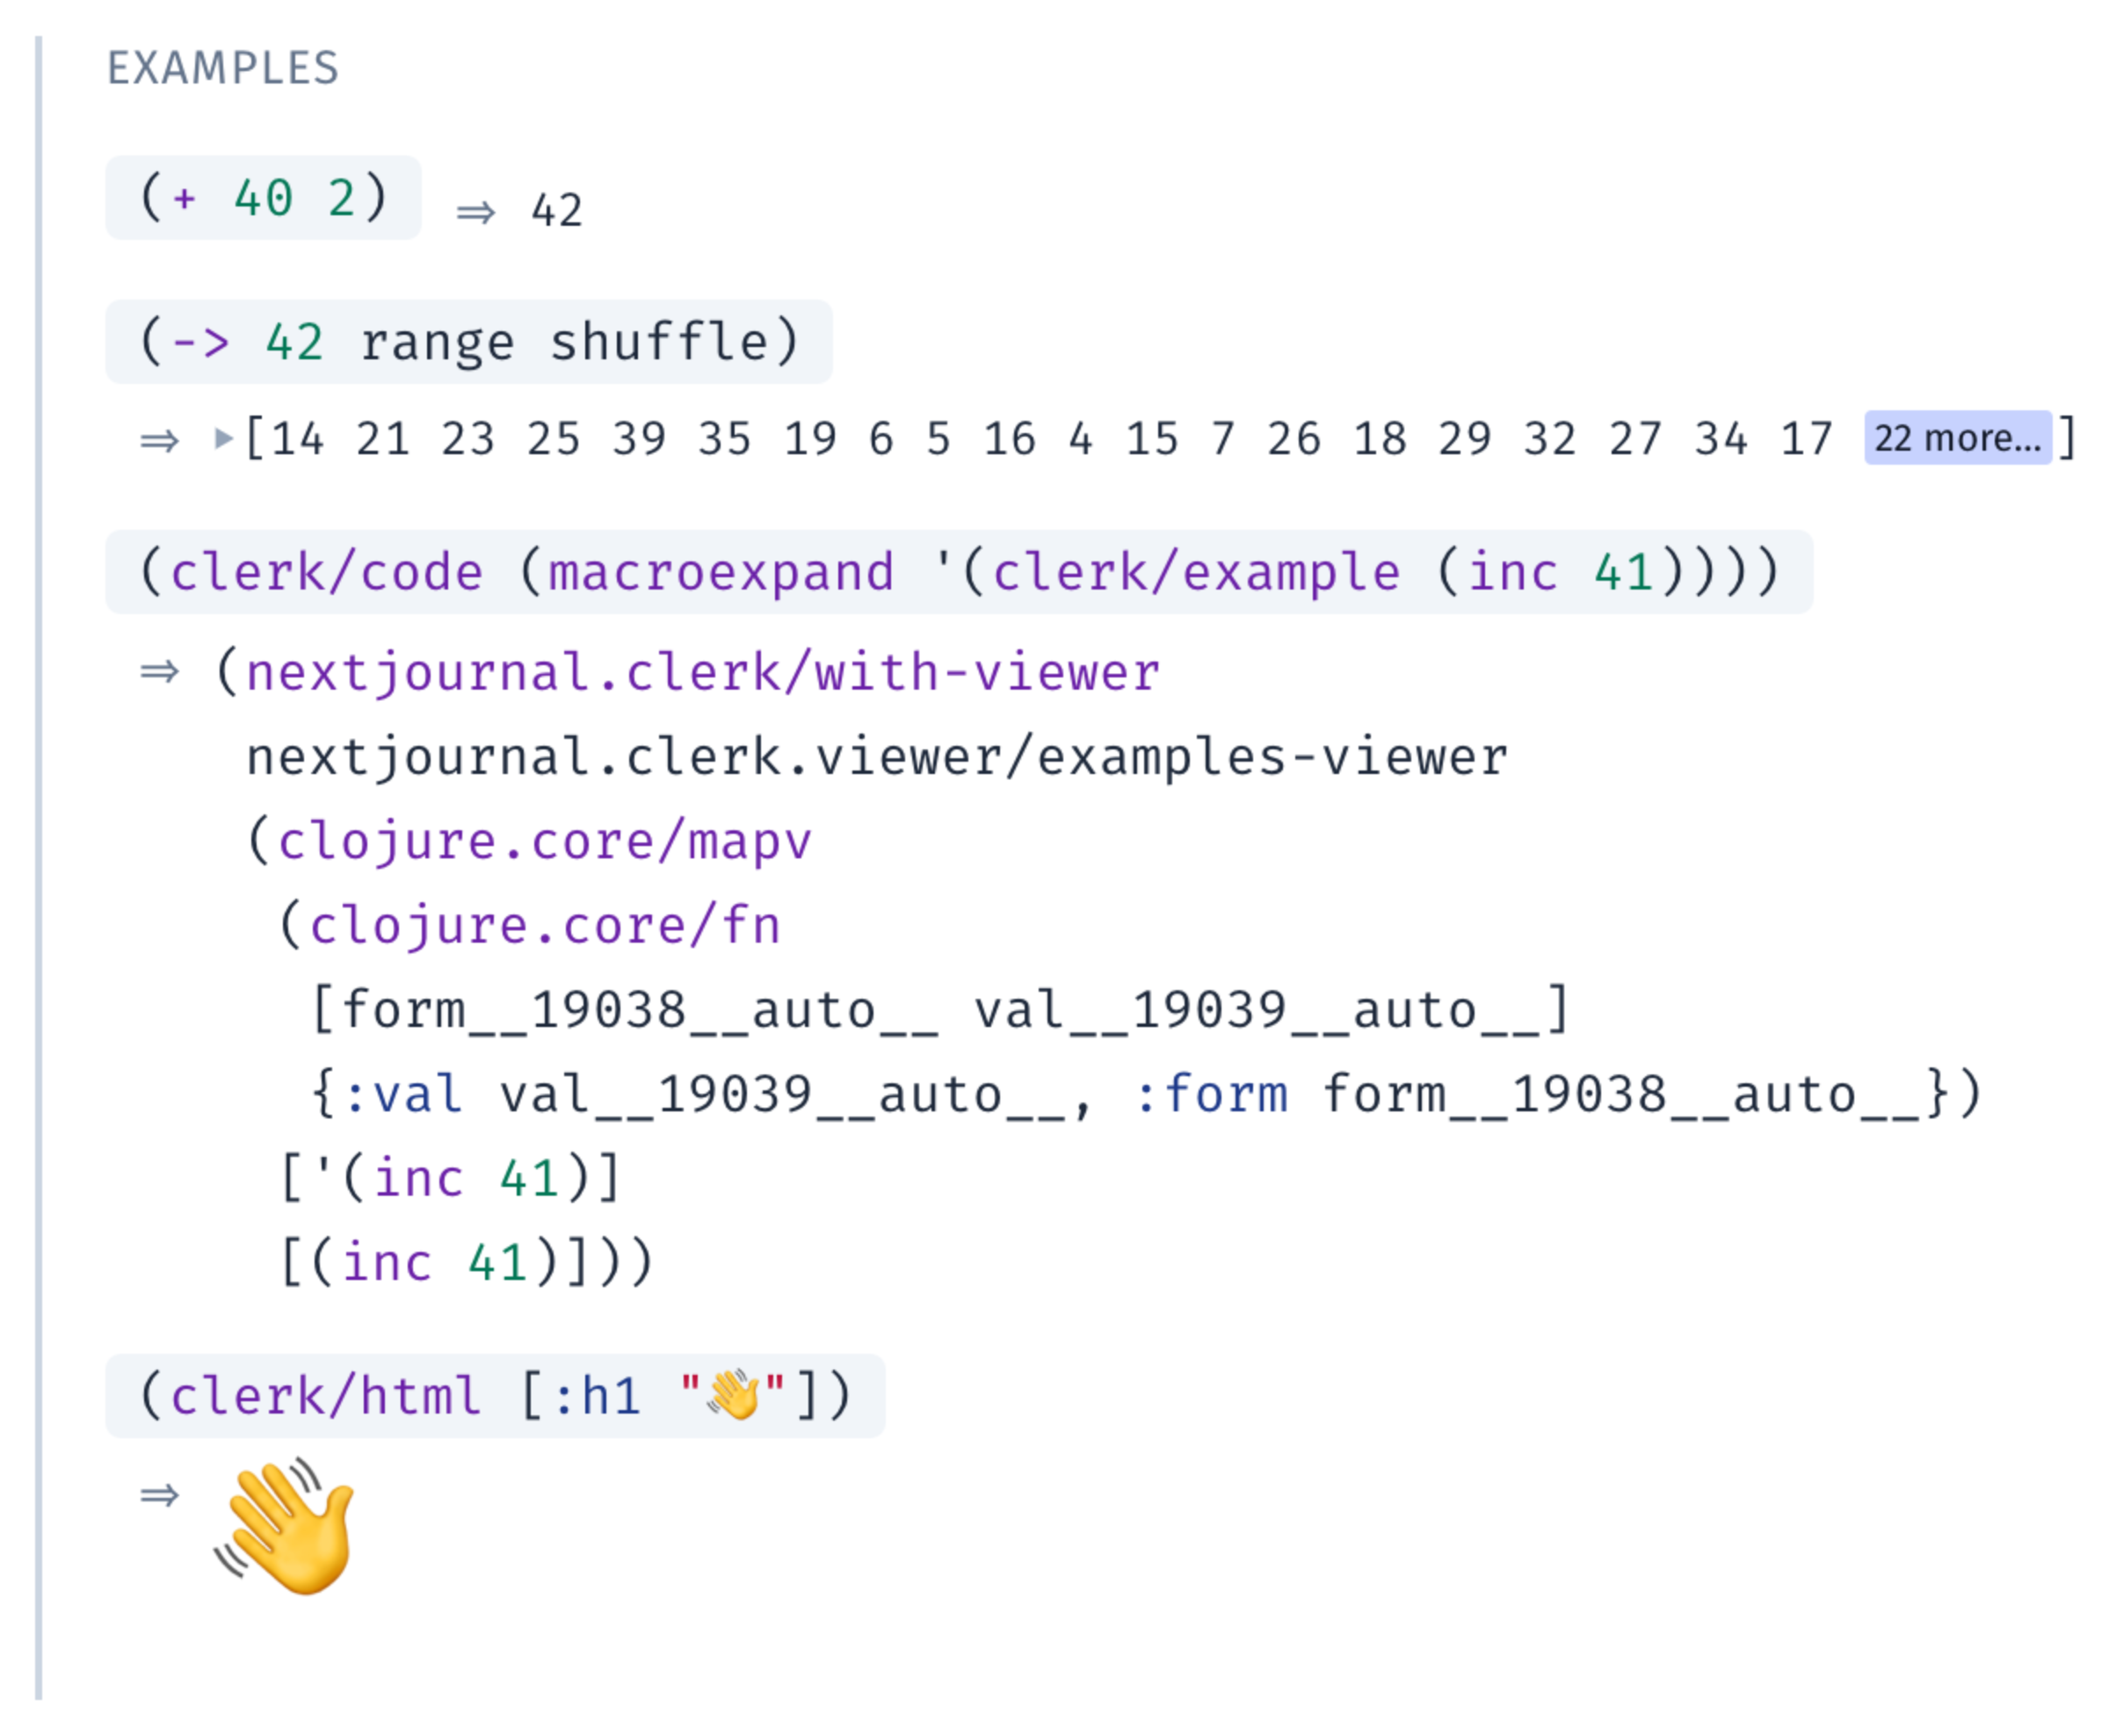
\includegraphics{images/anon-expr-5dtPQwixfSw57U4Tdiwqwrsj2tVHu1-result.png}

\hypertarget{prose-oriented-documents}{%
\subsection{Prose-Oriented Documents}\label{prose-oriented-documents}}

The first and primary use case for Clerk was adding prose, visualizations, and interactivity to Clojure namespaces. However, when writing documents that are mainly prose, but would benefit from \emph{some} computational elements, it is rather tedious to write everything in comment blocks. To make this easier, Clerk can also operate on markdown files with ``code-fenced'' source code blocks. All Clojure source blocks in such a file are evaluated and replaced in the generated document with their result.

This format is very similar to other markdown-based notebooks, like {\href{https://rmarkdown.rstudio.com}{R Markdown}\footnote{https://rmarkdown.rstudio.com}}, but specifically tailored to Clojure. We used this approach to write this paper, the source for which is located {\href{https://github.com/mk/clerk-px23}{on Github}\footnote{https://github.com/mk/clerk-px23}}.\footnote{One nice thing about this approach is that other systems, like Github, are able to render a reasonable version of the document, though without evaluation.}

During the review process for this paper, one of the reviewers mentioned that they would have preferred a PDF document to a website. We took this is an opportunity to test the flexibility of our system, adding a LaTeX translation layer to produce a separate printable version. It sadly lacks the interactive features of the web presentation, but we are quite pleased with the quality of the document we were able to send to press with relatively little additional work.

\hypertarget{examples-of-moldable-development-with-clerk}{%
\section{Examples of Moldable Development with Clerk}\label{examples-of-moldable-development-with-clerk}}

In addition to the sorts of traditional data science use cases that one might expect from something that has ``notebook" features, we intend Clerk to be a general purpose programmer\textquotesingle s assistant\footnote{We use this term in appreciation of pioneering historical work by Warren Teitelman.} that allows the rapid construction of tiny interfaces during daily work. Here are a few samples of tools and documentation created in this manner.

\hypertarget{augmenting-table-names}{%
\subsection{Augmenting Table Names}\label{augmenting-table-names}}

This example illustrates an approach we used to make working with a legacy DB2 database easier. The database's column names are made up of largely human-unreadable 8 character sequences:

\begin{figure}
\hypertarget{as400-column-names}{%
\centering
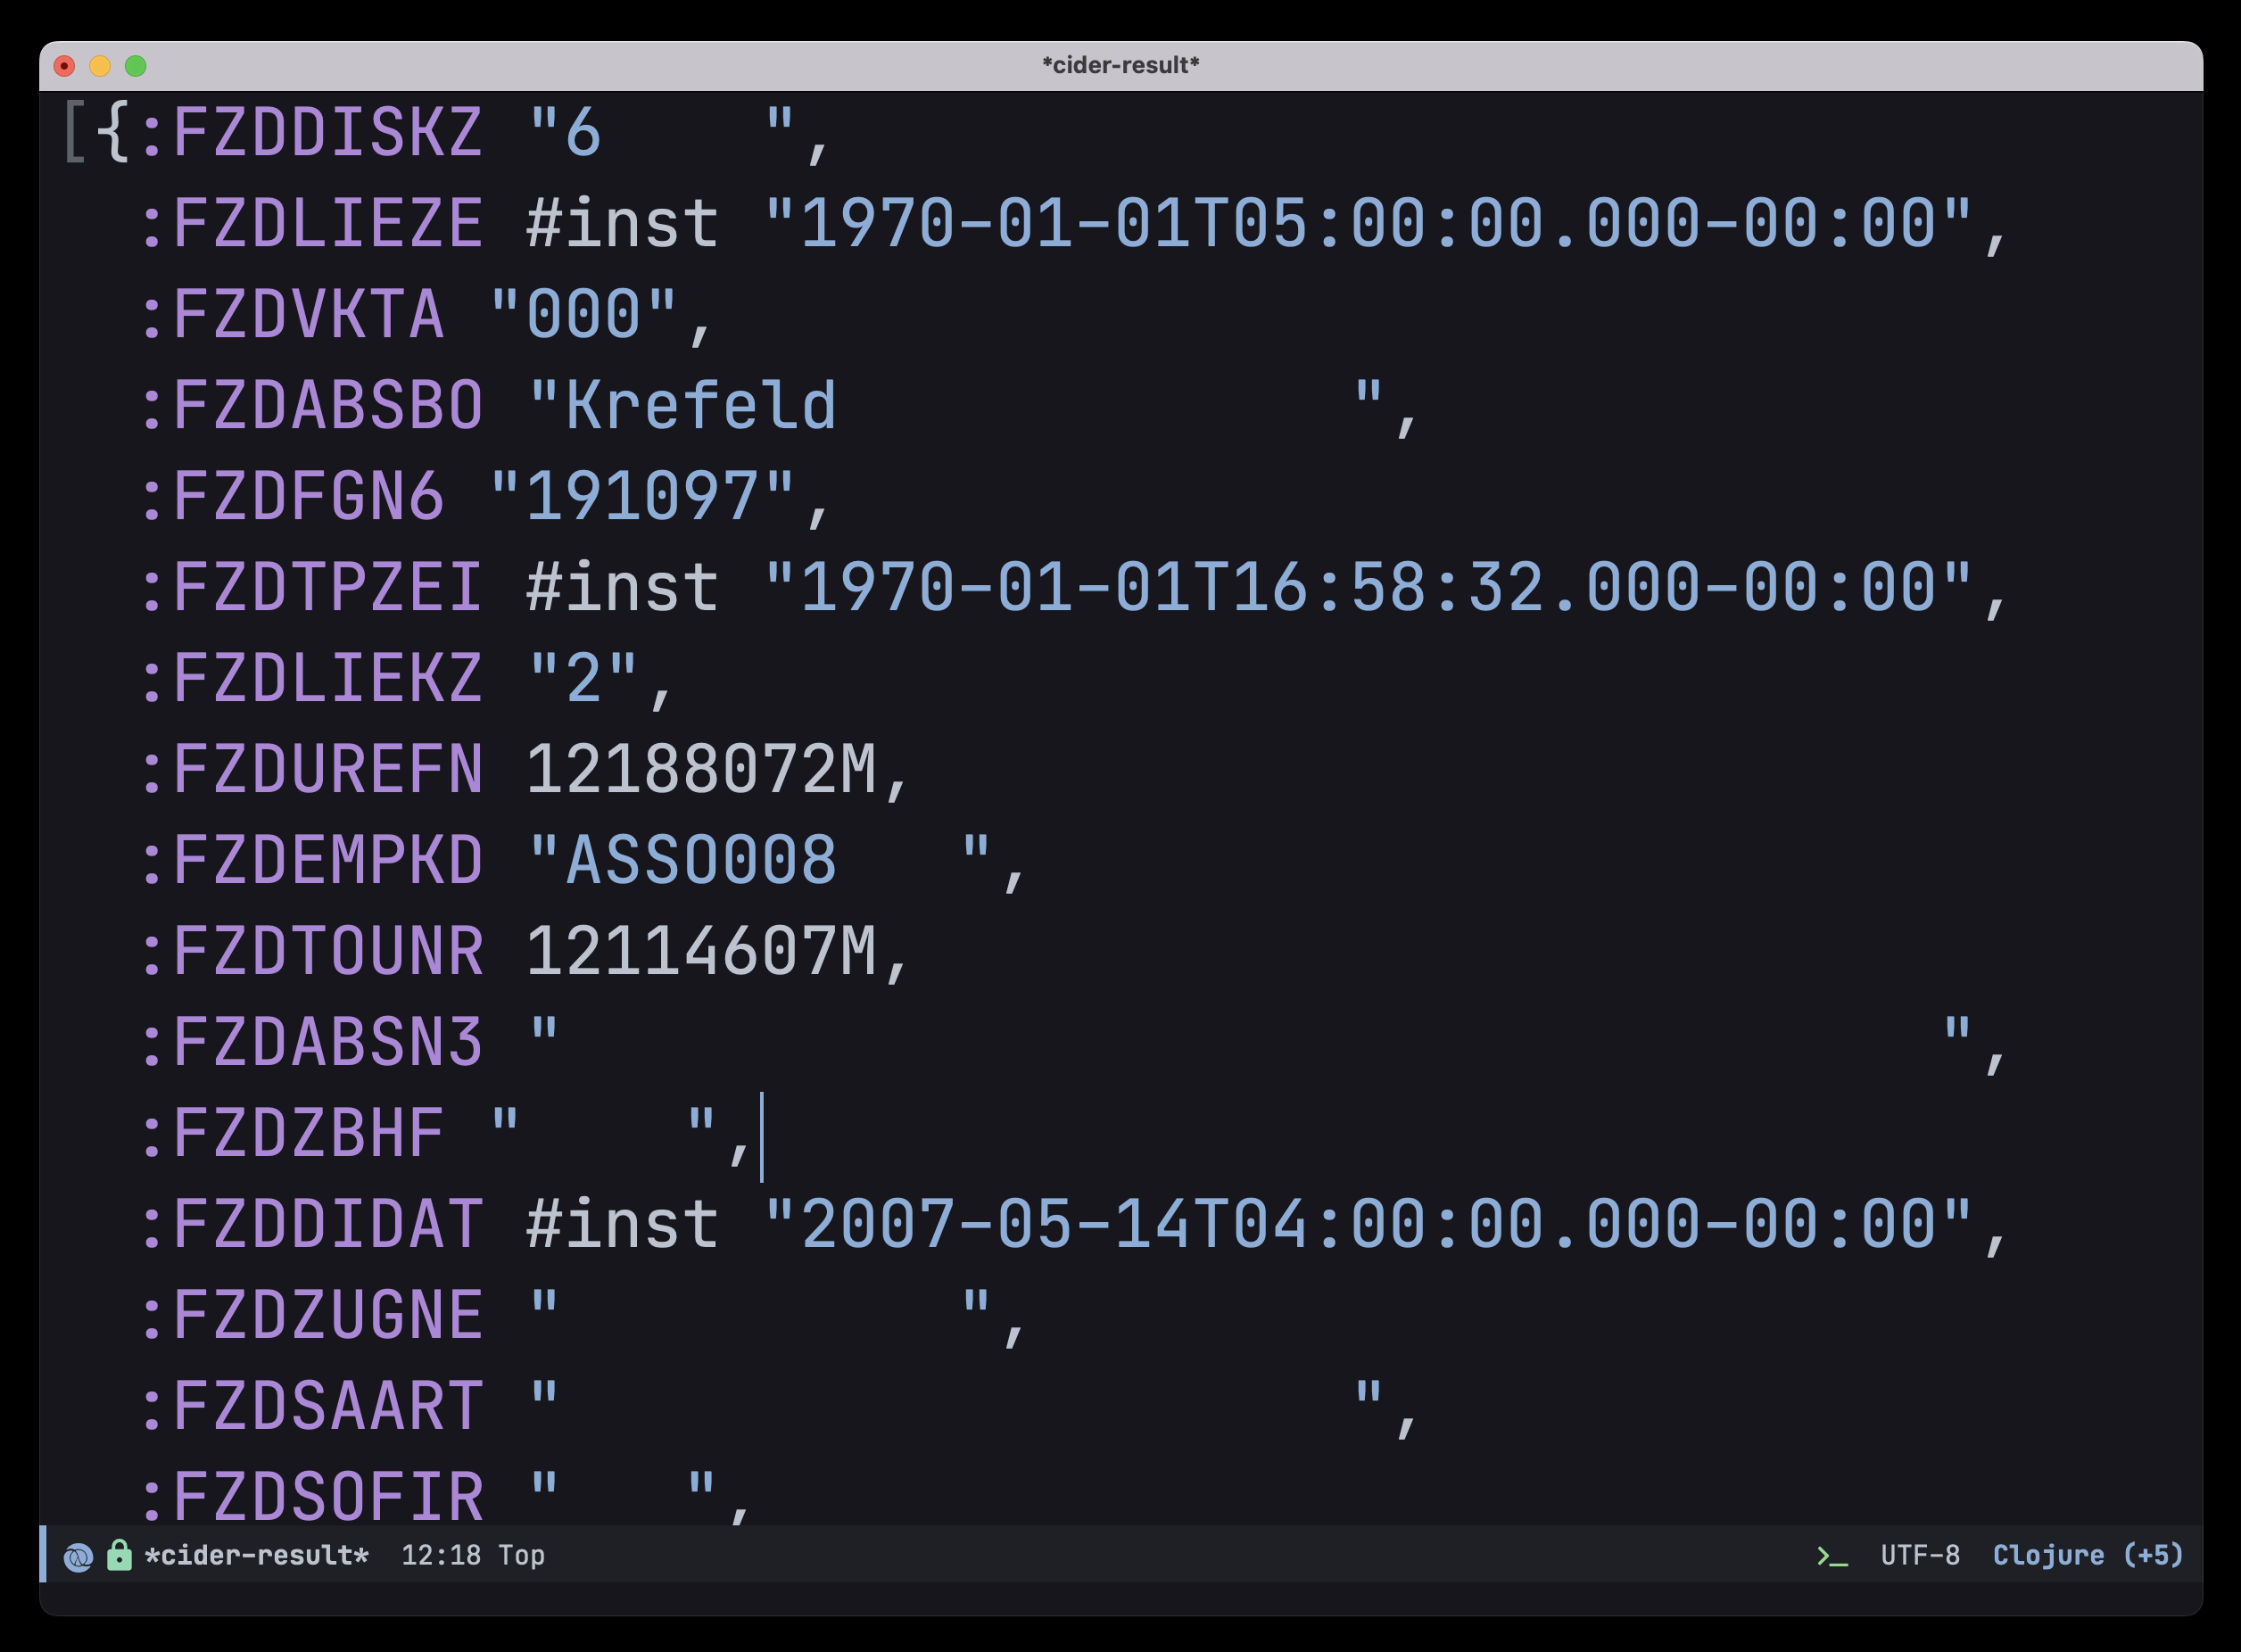
\includegraphics{images/QmWnzjc5c9qpUUaLoK3ytZk4Zs1AzDpZj1Tx5FF4ZR8a5t.png}
\caption{AS/400 Column Names}\label{as400-column-names}
}
\end{figure}

We were able to automatically translate these names using a metaschema extracted from the database. This allowed us to create a viewer that maps those eight-character names to human-readable (German-only) names (which we can then translate to English). In typical Lisp fashion, we go on to inspect a query interactively. We can use the translated names in the table, and even print them, but one quickly sees the limit of plain-text printing:

\begin{figure}
\hypertarget{inspecting-a-query-using-the-repl}{%
\centering
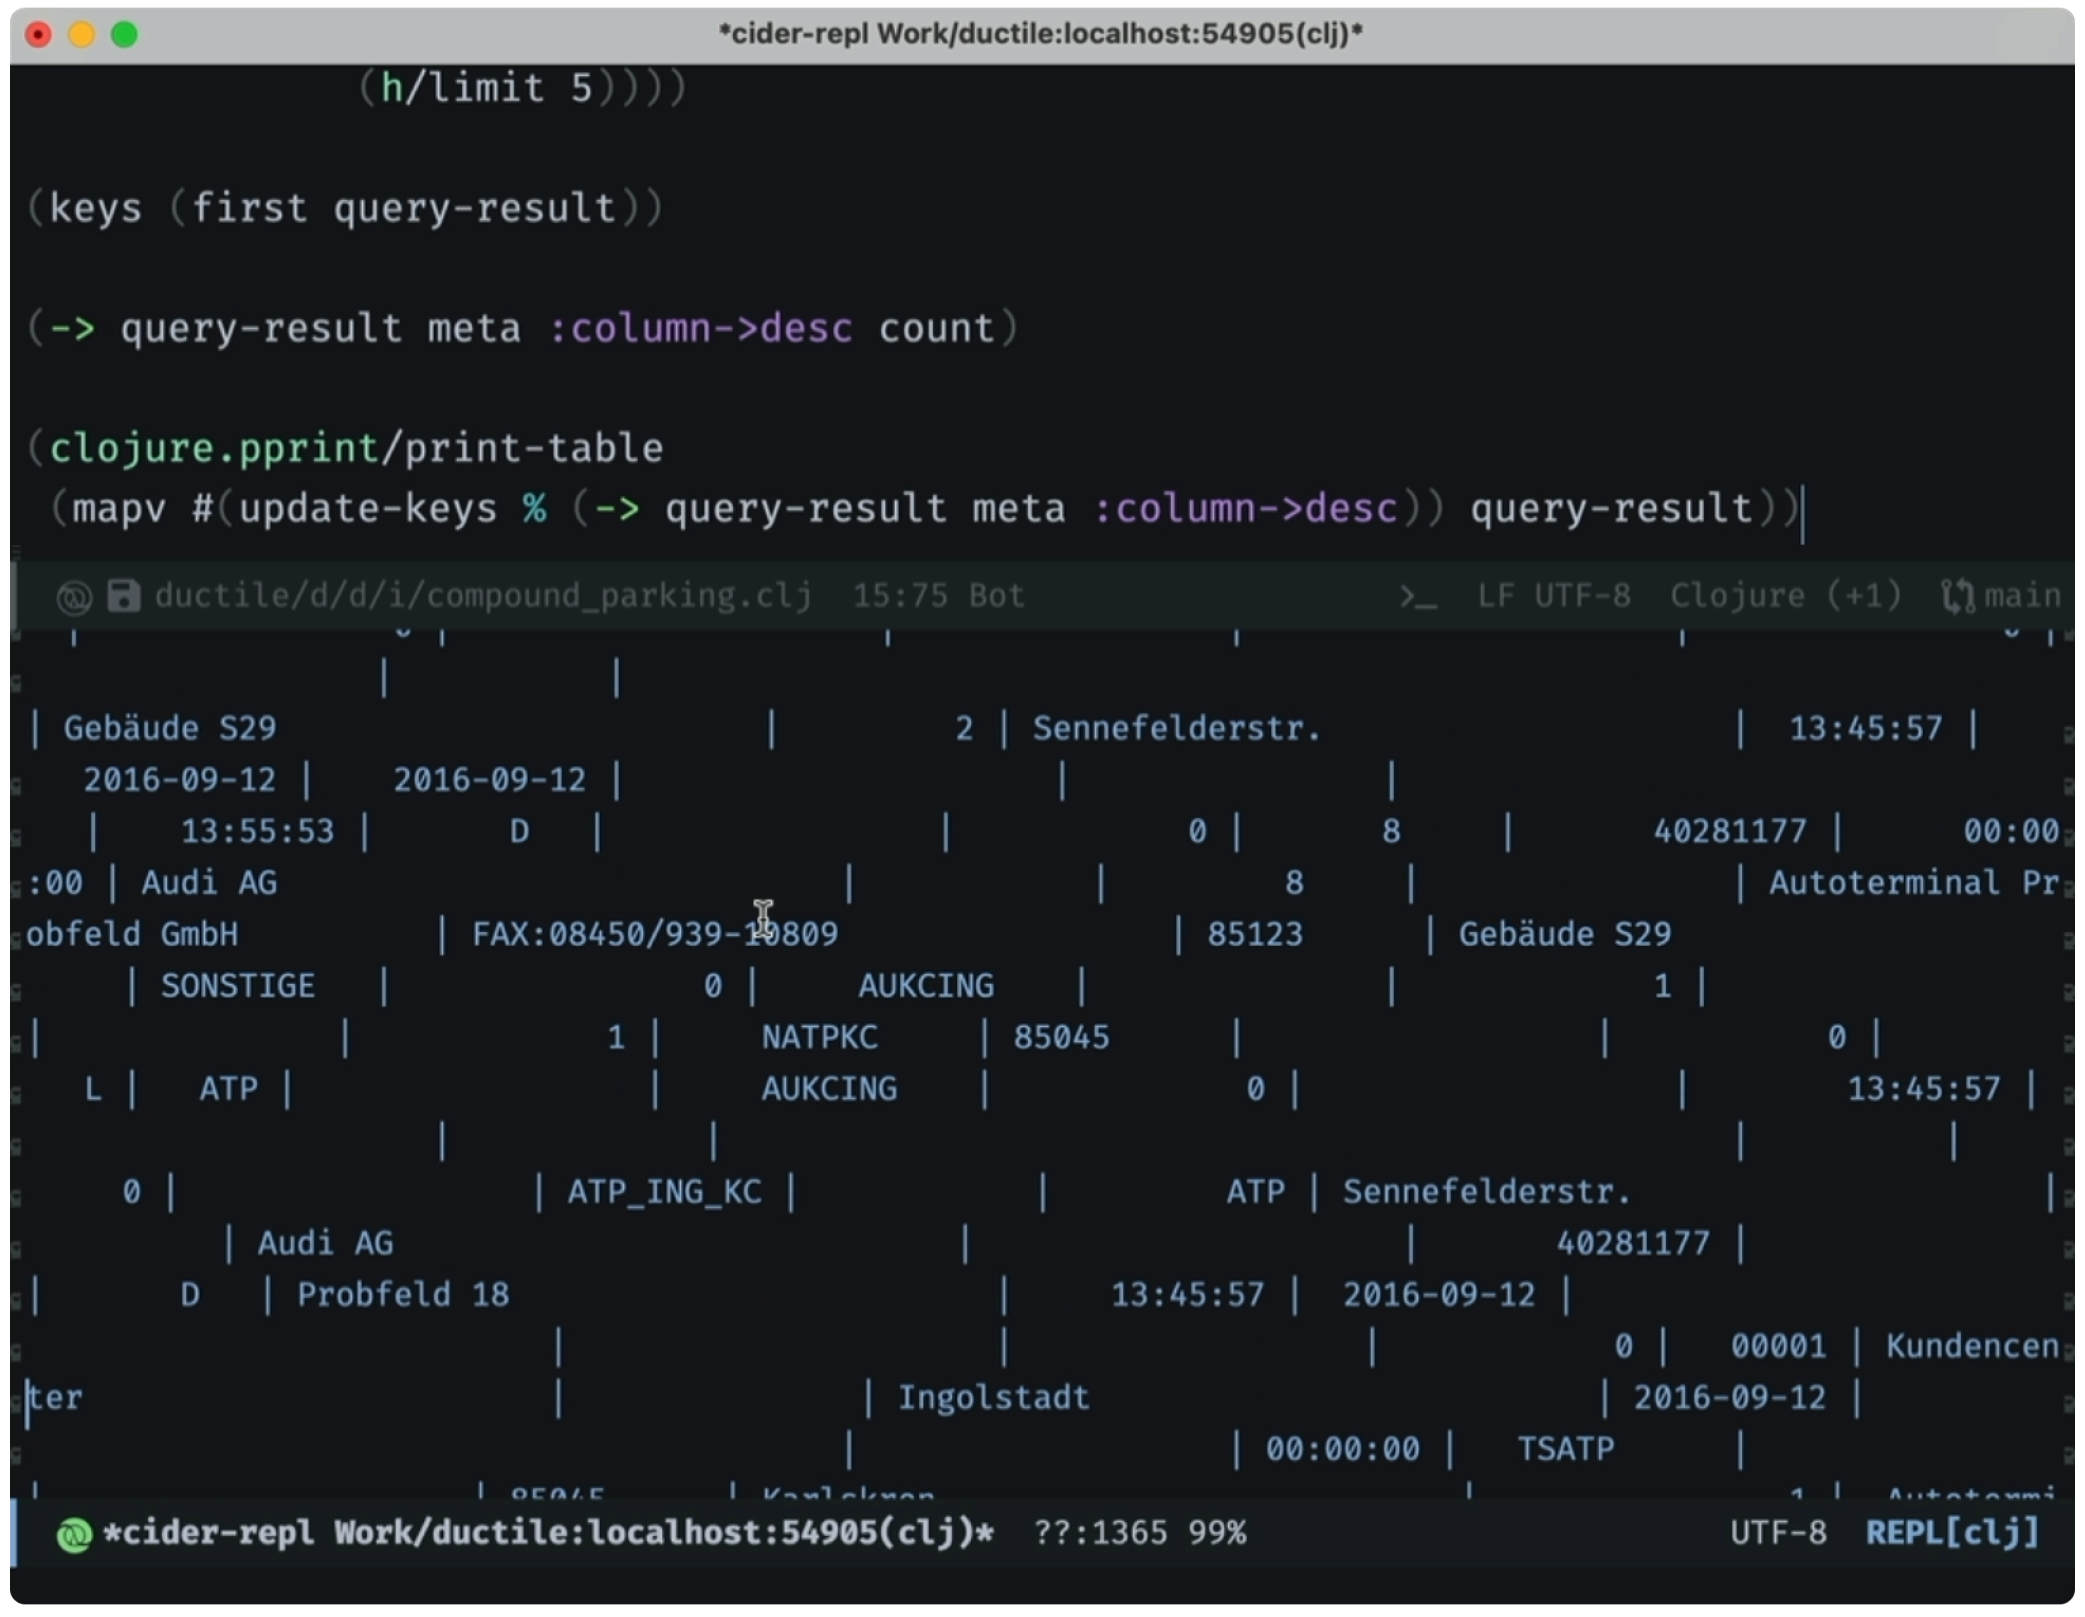
\includegraphics{images/QmagkcNvHsscf3DEq18nuXi6z3u4CyQWGzaRLf1hUm5a32.png}
\caption{Inspecting A Query Using the REPL}\label{inspecting-a-query-using-the-repl}
}
\end{figure}

With Clerk, were able to render the output as a graphical table without the limitations of plain text. Further, we can use the Viewer API to extend the table viewer's headings to show the translated metaschema names (plus showing the original eight character names in a de-emphasized way so that they aren't lost). We can go further still, showing the original German names when move the mouse over the headings:

\begin{figure}
\hypertarget{augmented-table-headings}{%
\centering
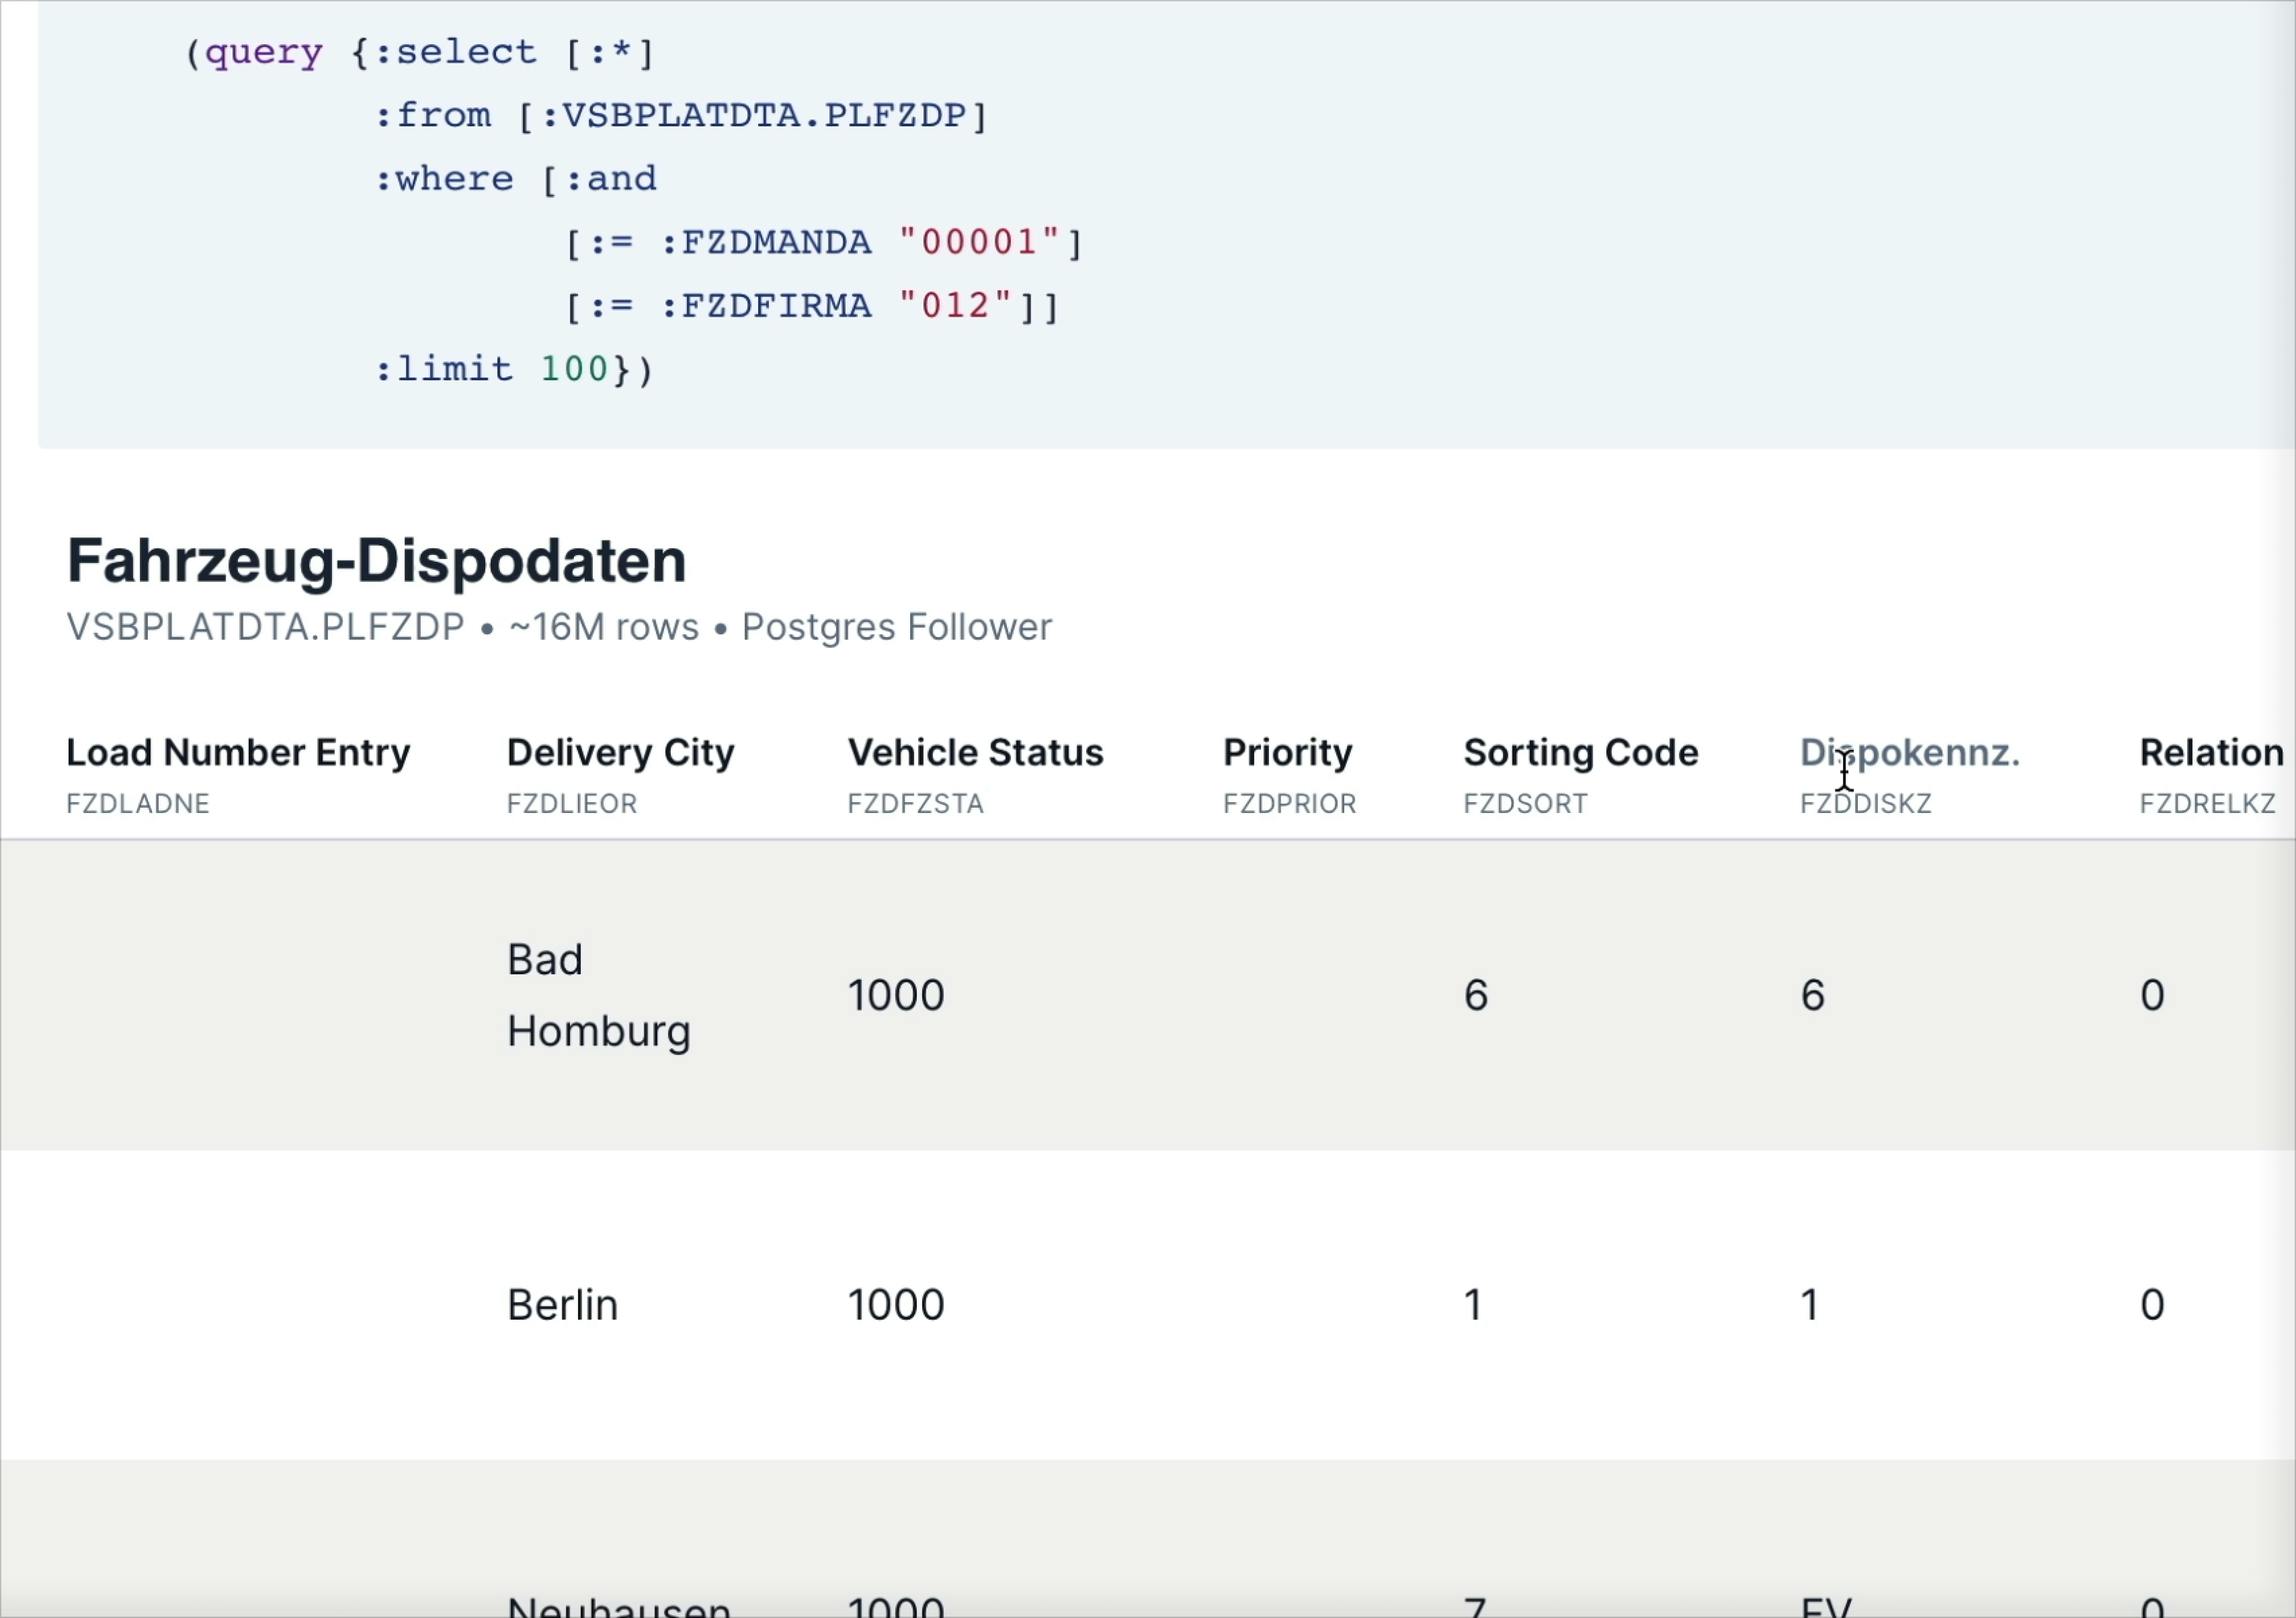
\includegraphics{images/QmVdGBFtcK7AAksAzmCH4t18f1RvCbepLZPixaq4ncz4cq.png}
\caption{Augmented Table Headings}\label{augmented-table-headings}
}
\end{figure}

\hypertarget{rich-documentation-features}{%
\subsection{Rich Documentation Features}\label{rich-documentation-features}}

This example illustrates the use of Clerk to create rich documentation for \passthrough{\lstinline!clojure2d!}'s colors package.\footnote{The full documentation is\\
  {\href{https://clojure2d.github.io/clojure2d/docs/notebooks/notebooks/color.html}{here} (https://clojure2d.github.io/clojure2d/docs/notebooks/notebooks/color.html)}.} They used Clerk's Viewer API to implement custom viewers to visualize colors, gradients and color spaces, then publish that documentation on the web by generating a static website directly from the source code of the library.

\begin{figure}
\hypertarget{custom-viewers-for-clojure2ds-colors-library}{%
\centering
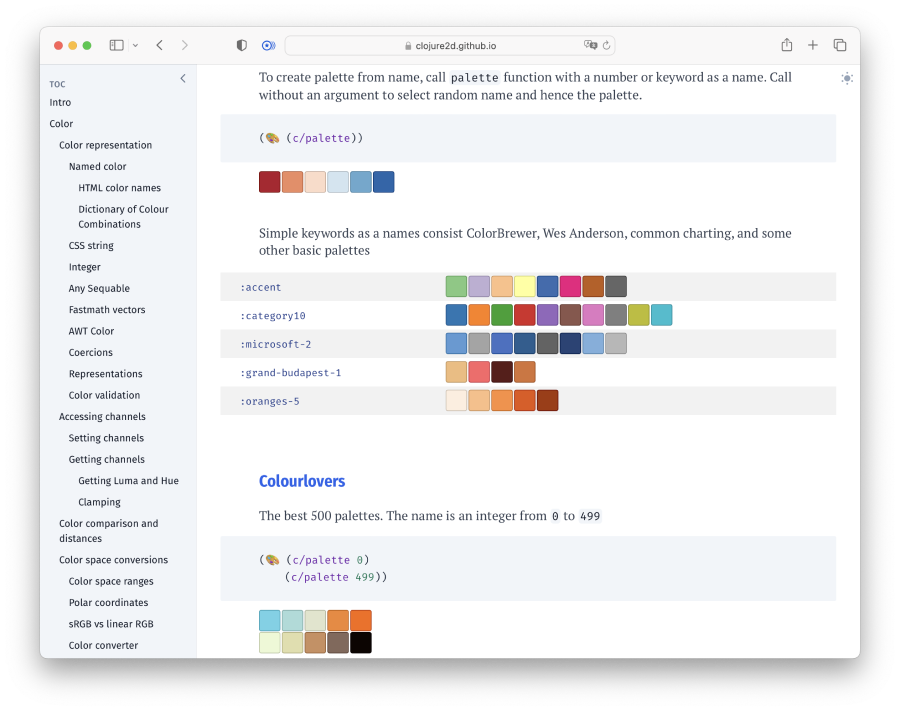
\includegraphics{images/QmQZ5kZwRYEEXUfNfWPsaidpoN88ugdSXYqEUVT5q1FyAE.png}
\caption{Custom Viewers for Clojure2d's Colors Library}\label{custom-viewers-for-clojure2ds-colors-library}
}
\end{figure}

\hypertarget{regex-dictionary}{%
\subsection{Regex Dictionary}\label{regex-dictionary}}

Built as a showcase for Clerk's sync feature, this example allows entering a regex into a text input and get dictionary matches as result while you type:

\begin{figure}
\hypertarget{interactive-regex-dictionary}{%
\centering
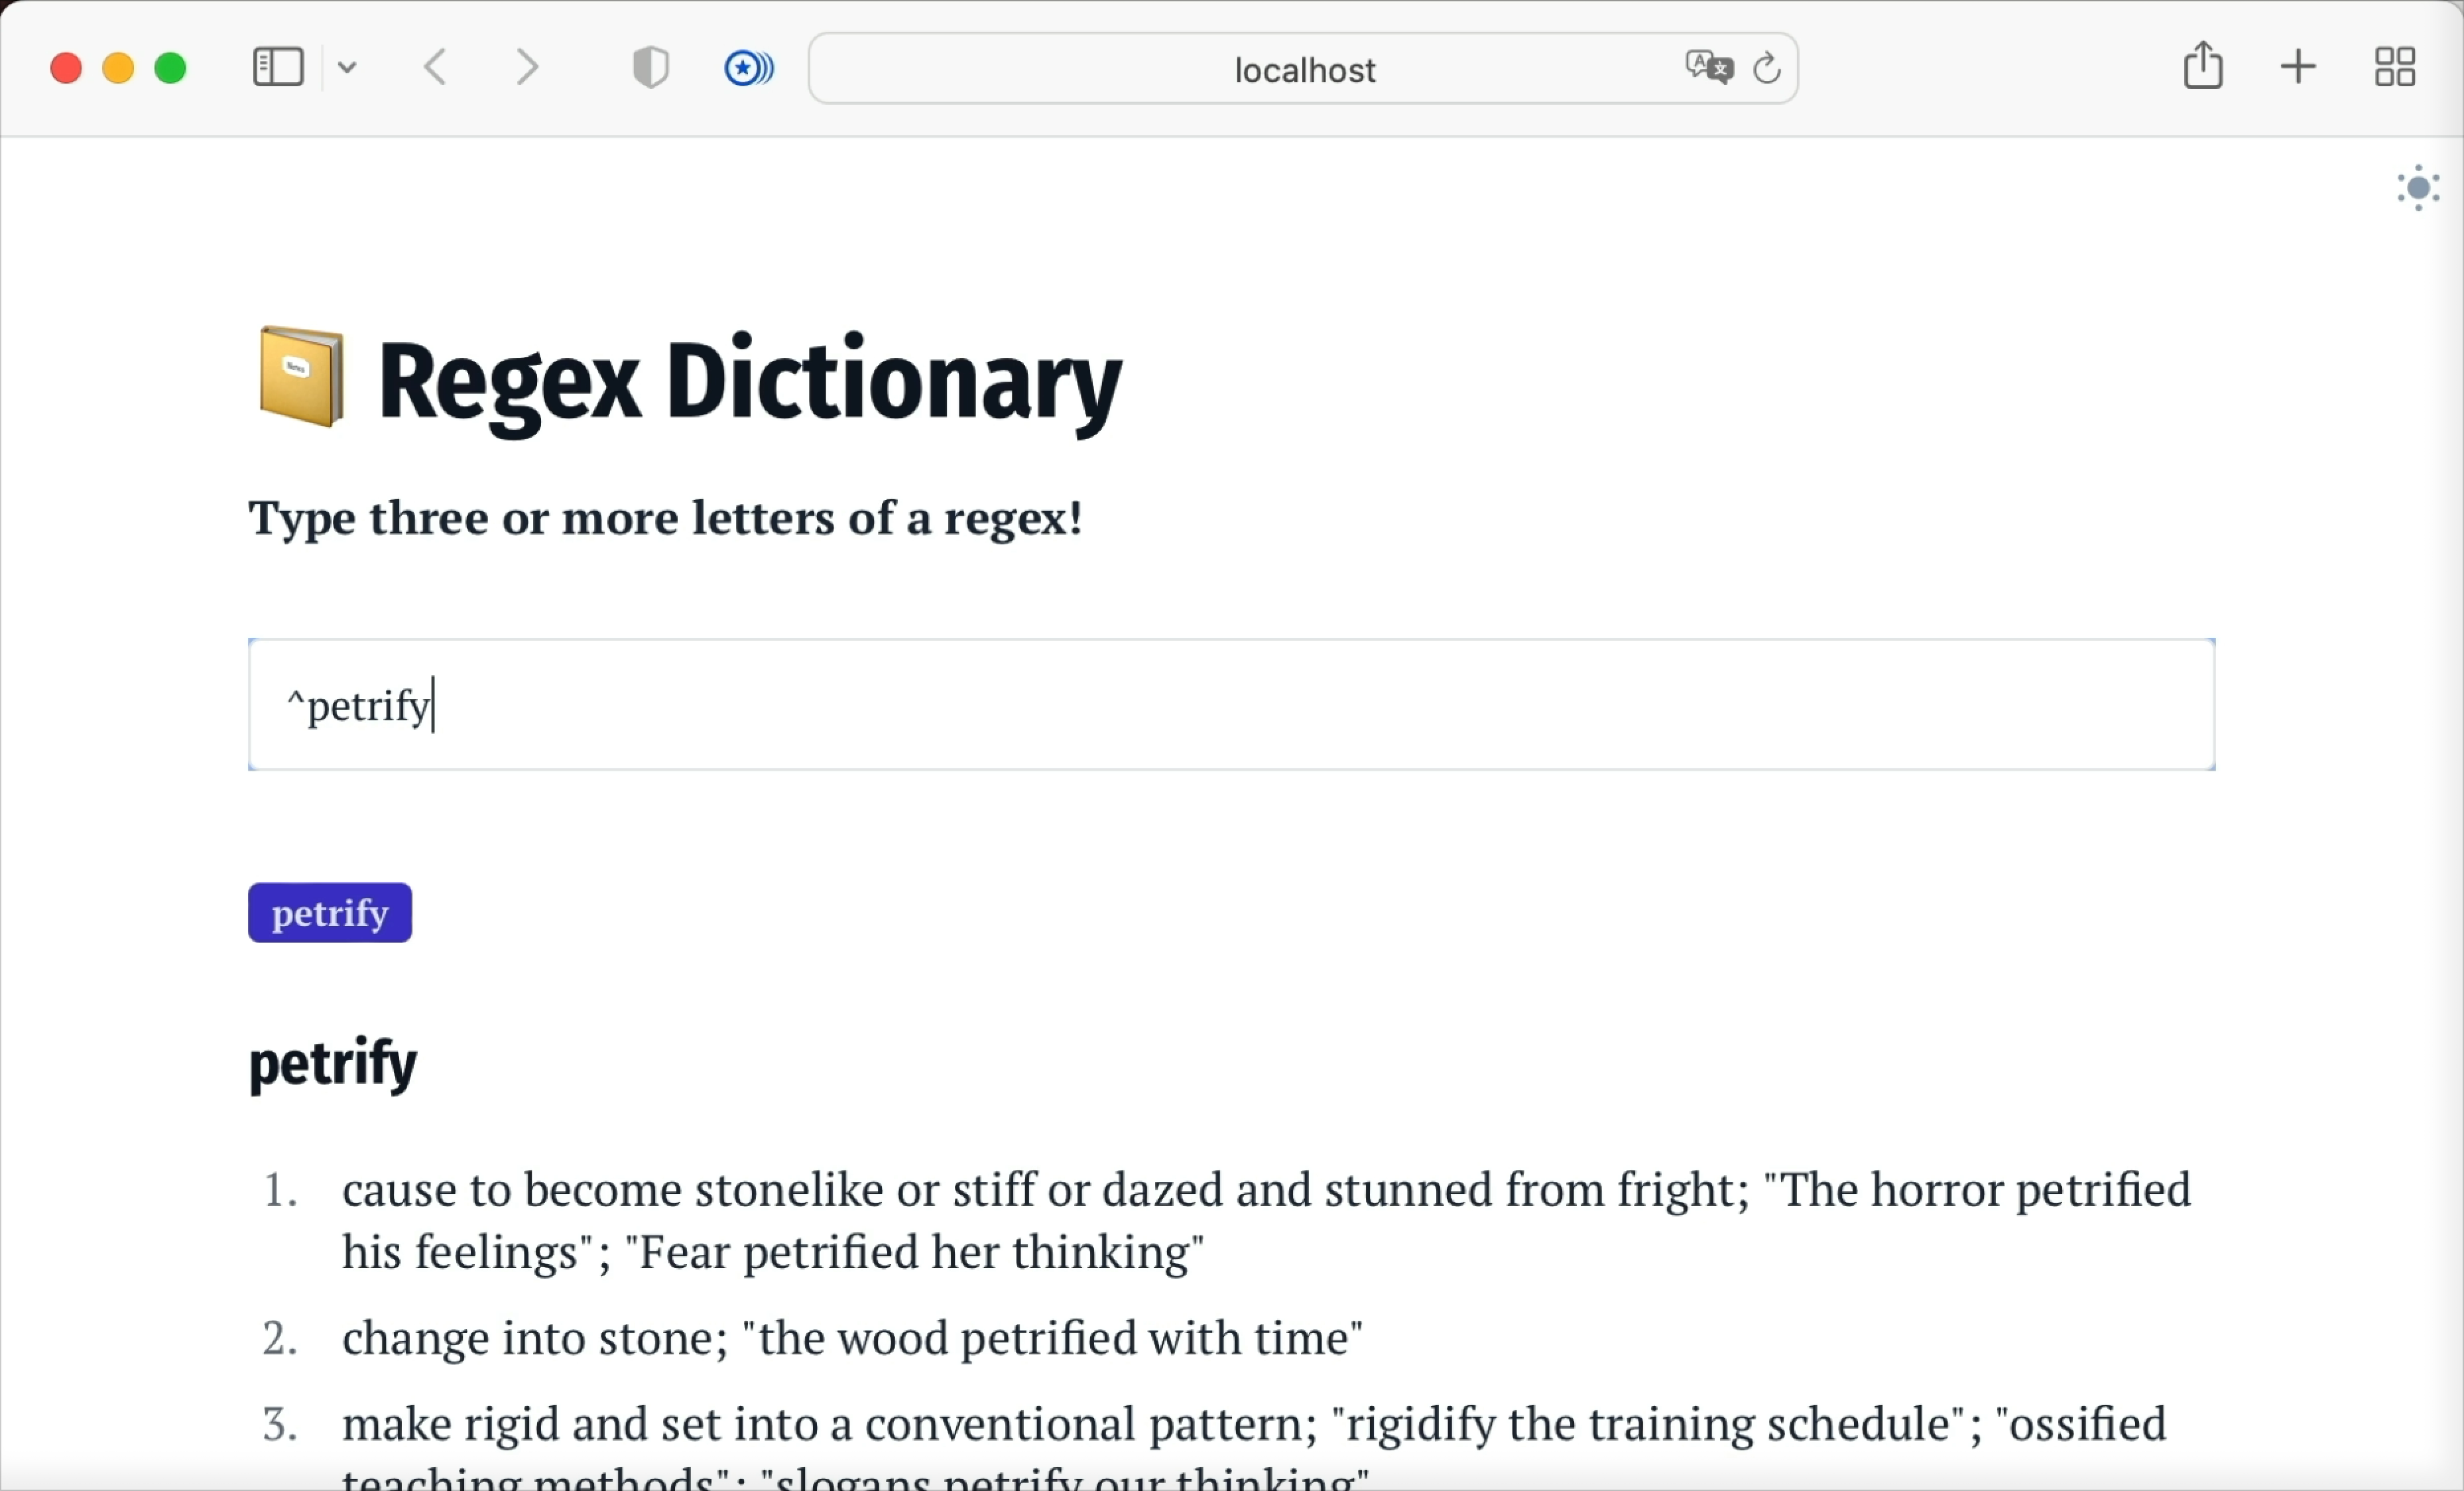
\includegraphics{images/QmWo1npCDCK5F1t7Aofc65pbbeMfoQNMVje4F6UMTBK4CK.png}
\caption{Interactive Regex Dictionary}\label{interactive-regex-dictionary}
}
\end{figure}

It is built using a Clojure atom containing the text input's current value that is synced between the client and server. As you type into the input, the atom's content will be updated and synced. Consequently, printing the atom's content in your editor will show the input's current value:

\begin{figure}
\hypertarget{printing-the-value-of-a-synced-clojure-atom}{%
\centering
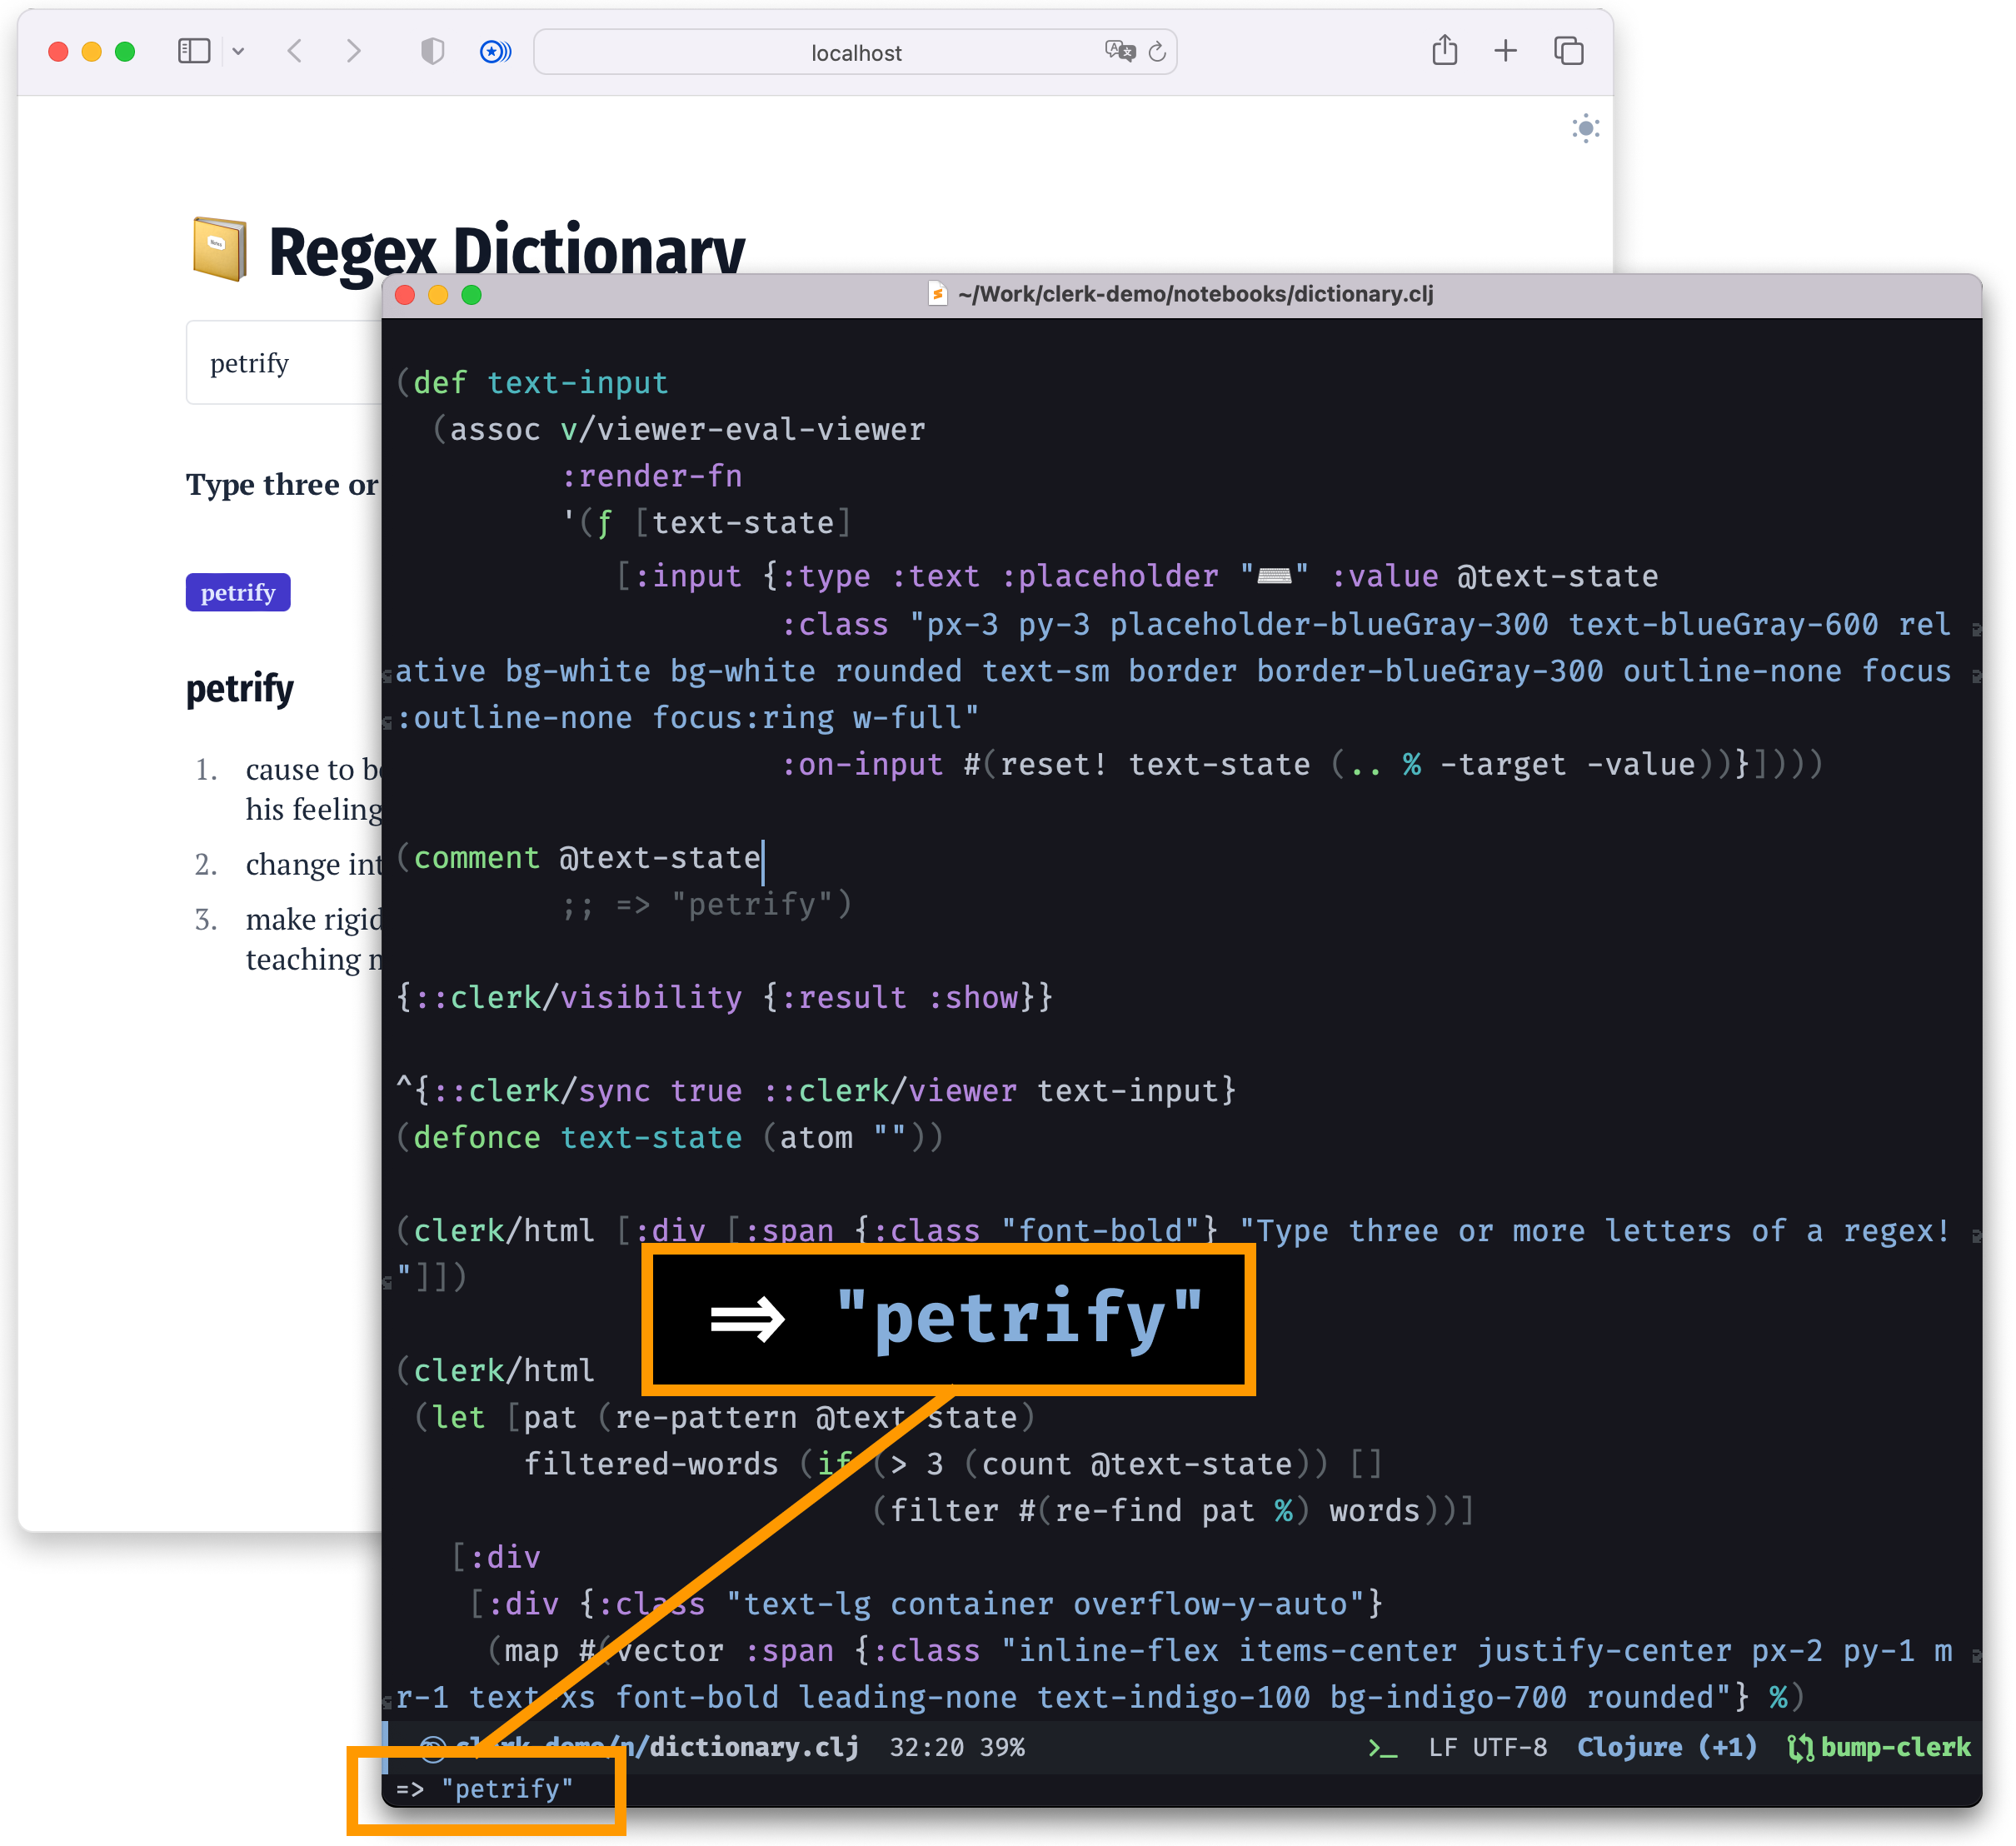
\includegraphics{images/QmRvfwCT5wJCbU8ALLghhD7v9chKob8MXcUV3vAf6XTbm8.png}
\caption{Printing the value of a synced Clojure atom}\label{printing-the-value-of-a-synced-clojure-atom}
}
\end{figure}

\hypertarget{lurk:-interactive-lucene-powered-log-search}{%
\subsection[: Interactive Lucene-Powered Log Search]{\texorpdfstring{{\href{https://github.com/nextjournal/lurk}{Lurk}\footnote{https://github.com/nextjournal/lurk}}: Interactive Lucene-Powered Log Search}{Lurk: Interactive Lucene-Powered Log Search}}\label{lurk:-interactive-lucene-powered-log-search}}

Also building on Clerk's sync feature, this interactive log search uses {\href{https://lucene.apache.org/}{Lucene}\footnote{https://lucene.apache.org/}} on the JVM side to index and search a large number of log entries. In addition to using query input, logs can also be filtered by timeframe via an interactive chart. It is worth noting that this example uses a full-screen layout by opting out of Clerk\textquotesingle s default notebook styling via Clerk's CSS customization options.

\begin{figure}
\hypertarget{interactive-log-search}{%
\centering
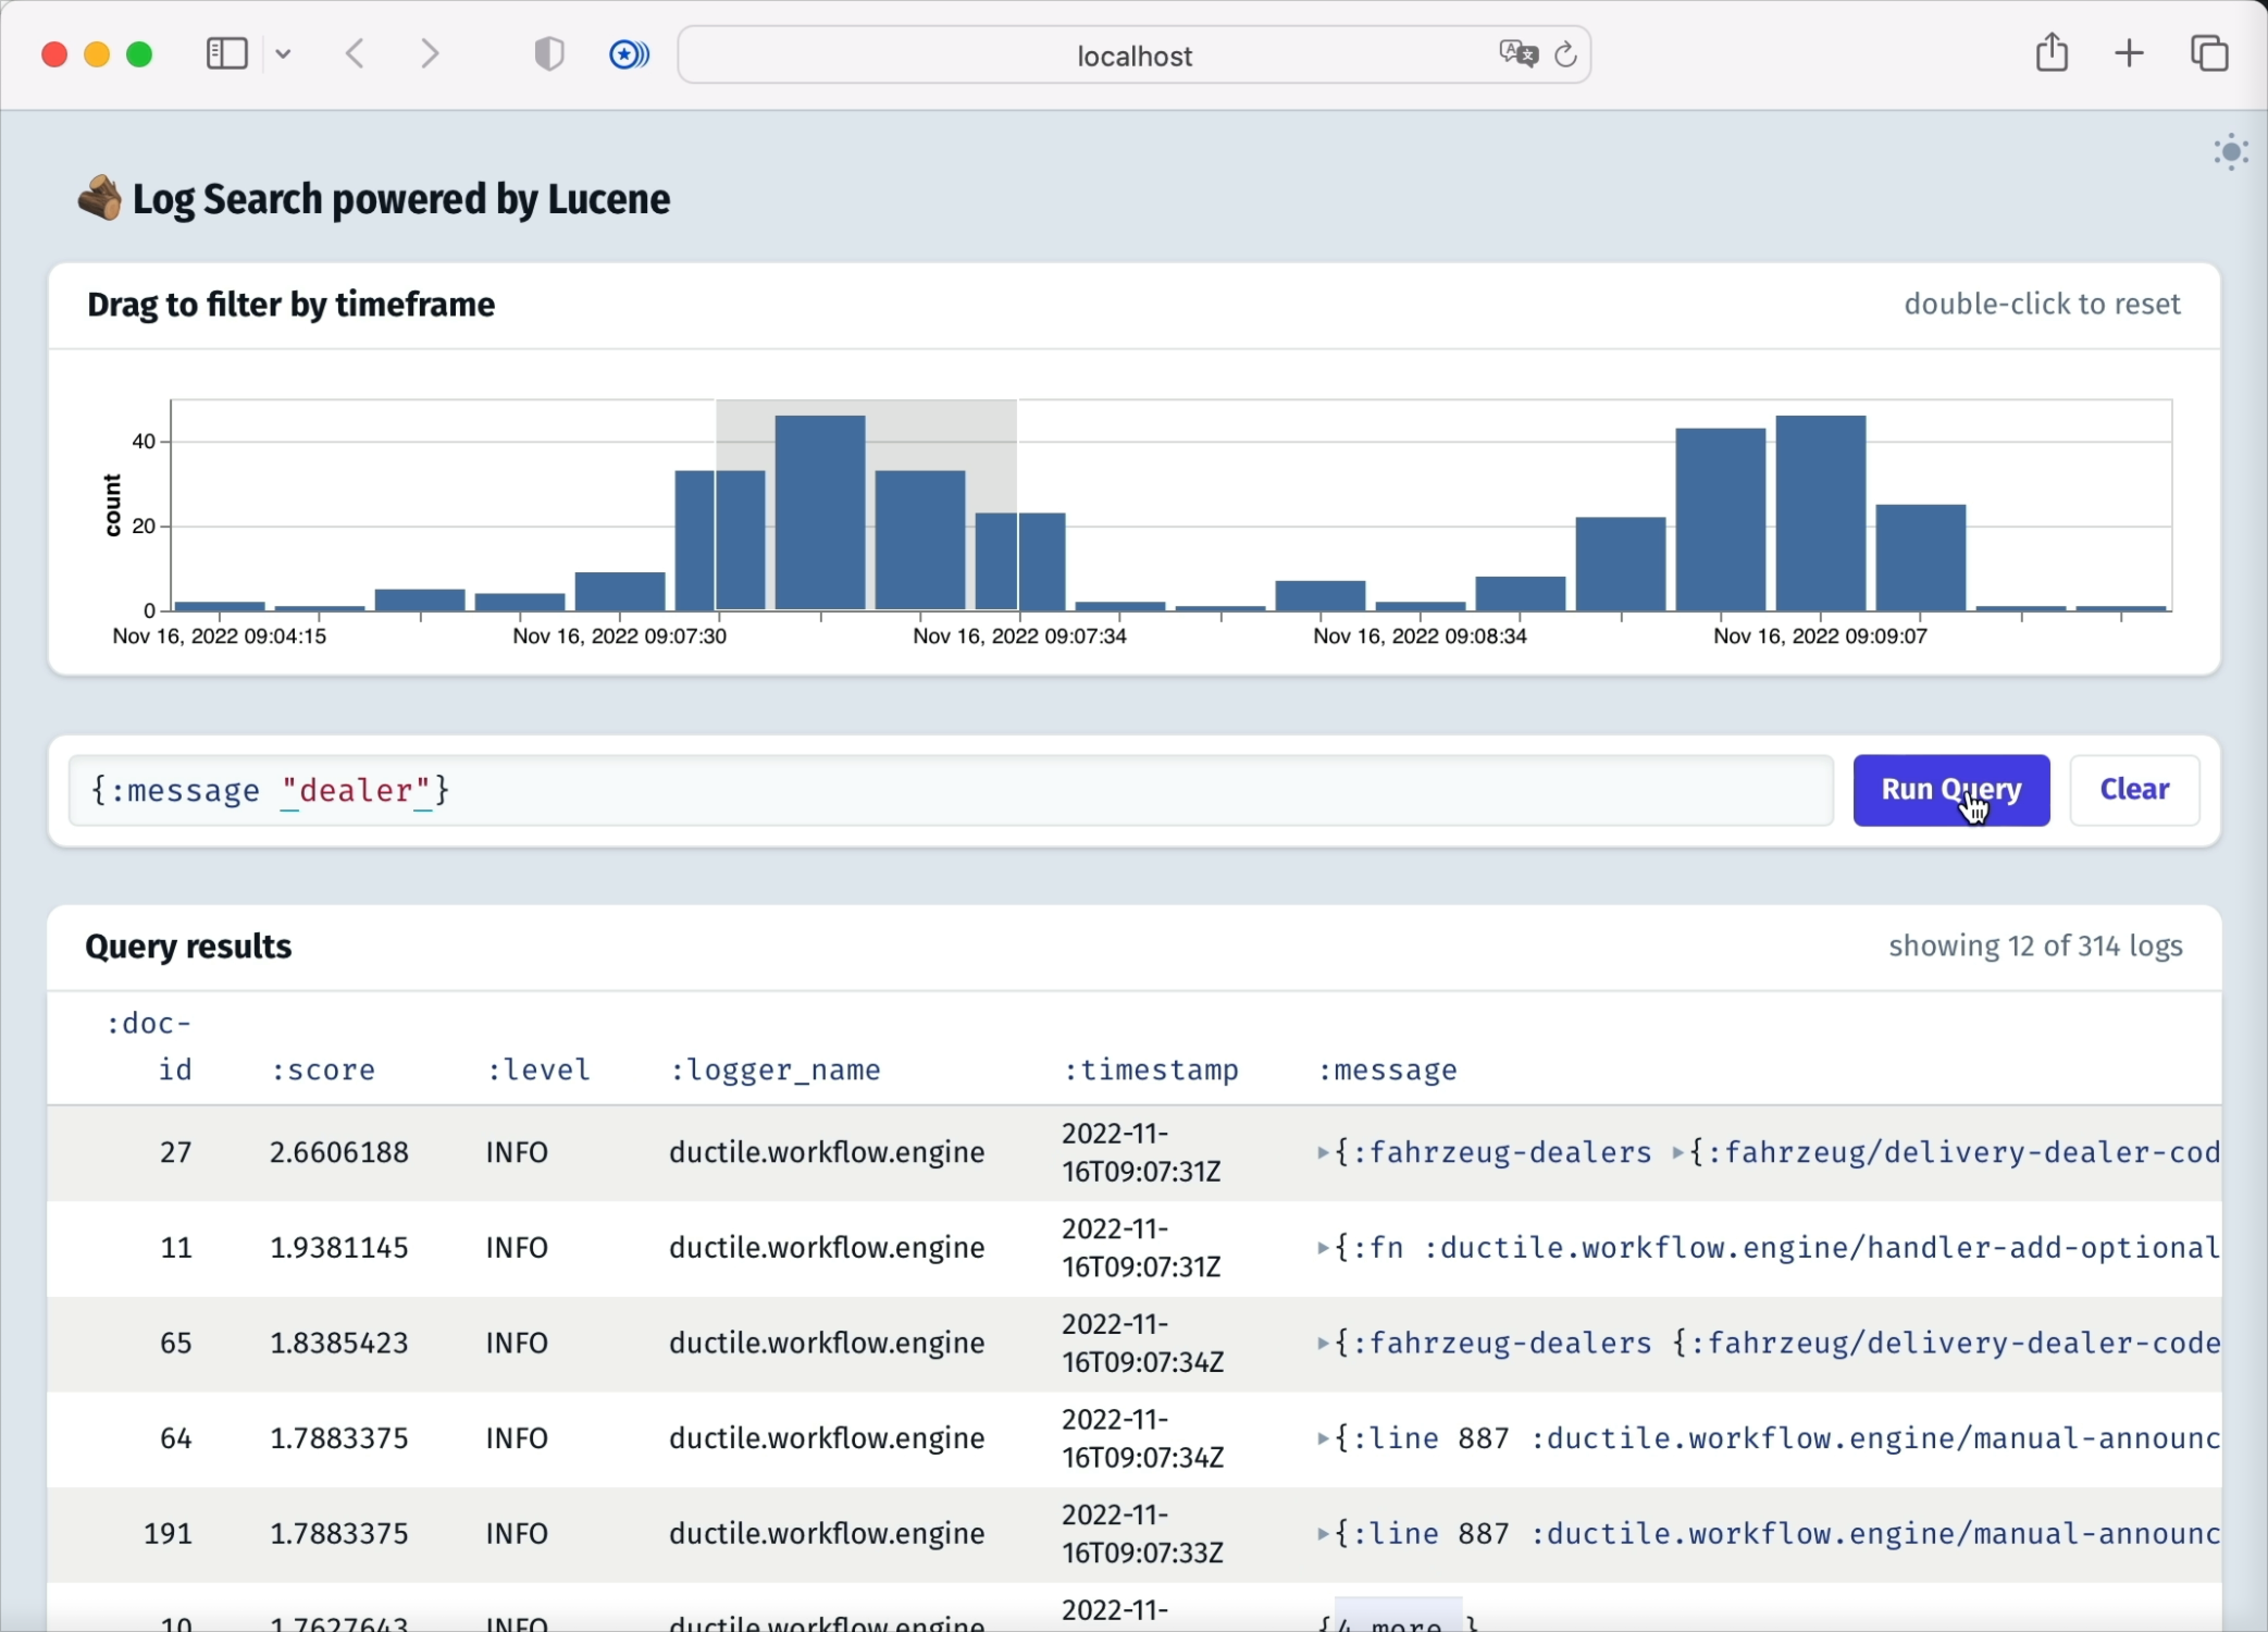
\includegraphics{images/QmcebVp6BGydcUUJhkjMurj5bBAdnDwbeiMjrmD6avKji4.png}
\caption{Interactive Log Search}\label{interactive-log-search}
}
\end{figure}

\hypertarget{experience}{%
\subsection{Experience}\label{experience}}

Our experience as the developers and users of Clerk has been surprisingly positive, and it has seen solid adoption within our organization, including many of us also using it for side-projects.

We believe this is in large part due to the purely additive design of Clerk. When one chooses to view a namespace through Clerk, it evokes feelings of added power, without the loss of control that comes from leaving one\textquotesingle s comforting and familiar editing environment (Emacs, Vim, VS Code). In hindsight, we now realize that we underestimated what a big ask that is for potential users of these sorts of systems.

We\textquotesingle ve chosen a few quotes from Clerk\textquotesingle s user base to give a sense of how the Clojure community has experienced Clerk. So far, even with thousands of users, we\textquotesingle ve had mostly positive feedback, aside from the usual bug reports every project receives.

\begin{quote}
{[}Clerk{]} is making the training of junior Clojure programmers a massive pleasure! {[}...{]}

It helps us to bypass what would otherwise be a lot of distracting UI programming. Set up your env, make a namespace, hit a keybind, hey presto, your code is running in a browser.

--~Robert Stuttaford
\end{quote}

\begin{quote}
I\textquotesingle m using Clerk to visualize statistics properties from a simulation in a model checker {[}...{]} it\textquotesingle s basically a wrapper over TLA+ {[}...{]}

Amazing that Clerk just lets you focus on what really matters and nothing else!

--~Paulo Feodrippe
\end{quote}

\begin{quote}
I just wanted to express some gratitude for Clerk. It's been a game changer for me in terms of understanding problems and communicating that understanding to other people.

-- Jeffrey Simon
\end{quote}

One often under-appreciated area in the academic discourse on programming is aesthetics. We believe the baseline level of design that is automatically inherited by any document produced with Clerk has contributed to the positive experiences our users have reported.

\begin{quote}
Attractive things do work better---their attractiveness produces positive emotions, causing mental processes to be more creative, more tolerant of minor difficulties.

-- Don Norman, Emotional Design
\end{quote}

\hypertarget{related-work}{%
\section{Related Work}\label{related-work}}

Besides the systems mentioned earlier in the paper, there are a number of other contemporary related systems. Many of them introduce the viewing layer to the editor itself, as seen in various Smalltalk experiments (Moldable Development \cite{Chi__2015},  Newspeak\footnote{{\href{https://newspeaklanguage.org/pubs/newspeak-exemplars.pdf}{Enhancing Liveness with Exemplars in the Newspeak IDE} (https://newspeaklanguage.org/pubs/newspeak-exemplars.pdf)} by Gilad Bracha.},  Babylonian Programming \cite{Rauch_2019}, etc), and in recent work on LiveLits \cite{Omar_2021} and visual syntactic extensions to the Racket programming language. \cite{Andersen_2020}

In contrast, because we have found it more persuasive to argue for the use of such systems in the context of a user\textquotesingle s existing tooling, we\textquotesingle ve focused on an approach that supplements existing workflows with a sidecar previewer. Other systems that have taken a similar approach include:

\begin{itemize}
\item
  {\href{https://orgmode.org}{Org mode}\footnote{https://orgmode.org}} is a major mode for {\href{https://www.gnu.org/software/emacs/}{Emacs}\footnote{https://www.gnu.org/software/emacs/}} supporting polyglot literate programming based on a plain text format. Org\textquotesingle s approach is in many ways similar to our Markdown mode, where explicit code fences are used to introduce programmatic constructs to a document, and a variety of previewers are available for org files, though in a fragmented ecosystem where each kind of application requires a different kind of previewer. We were partially inspired by positive experiences using org-mode in the design of Clerk, though we focused more on our annotated source code format.
\item
  {\href{https://streamlit.io}{Streamlit}\footnote{https://streamlit.io}} is a Python library that eshews a custom format and enables building a web UI on regular python scripts. Its {\href{https://docs.streamlit.io/library/get-started/main-concepts\#caching}{caching system}\footnote{https://docs.streamlit.io/library/get-started/main-concepts\#caching}} memoizes functions that are tagged using Python\textquotesingle s decorators. While there are several similarities between Clerk and Steamlits, the two systems have a very different focus. Streamlit is primarily a rapid application development environment, without Clerk\textquotesingle s focus is on combining Literate Programming and Moldable Development.
\end{itemize}

We are pleased to see a number of other systems working with annotated source code, including {\href{https://plutojl.org}{Pluto}\footnote{https://plutojl.org}} and {\href{https://livebook.dev}{Livebook}\footnote{https://livebook.dev}}, and consider this convergent evolution toward tools that developers are more likely to actually use as a positive trend.

\hypertarget{future-work}{%
\section{Future Work}\label{future-work}}

Our goal with the development of Clerk is to \emph{leave the toolbox open}: we want Clerk\textquotesingle s users to be able to customize the behavior of the running system in a predictable way, often by providing functions to the system at runtime.

Clerk\textquotesingle s viewer API is a first example of this approach, but we want to take it further by letting users:

\begin{itemize}
\tightlist
\item
  provide functions to control the caching e.g. to support more efficient caching of data frames
\item
  letting the viewer API\textquotesingle s \passthrough{\lstinline!:pred!} function opt into receiving more context like the path in the tree
\item
  make caching more granular and support caching function invocations
\item
  override \passthrough{\lstinline!parse!} and \passthrough{\lstinline!eval!} to support additional syntaxes with different semantics
\end{itemize}

So far we\textquotesingle ve mainly used Clerk\textquotesingle s caching on local machines in isolation. We plan to share a distributed cache within our dev team in order to learn about the benefits and challenges this can bring. We also want to extend Clerk to better communicate caching behavior to its users (why a value could or could not be cached, if it was cached in-memory or on-disk).

We\textquotesingle re also actively exploring different ways of bringing an exploratory Clerk notebook to production. In exploratory work one often uses global state in Clojure atoms and vars which makes a computation tangible. When serving concurrent requests in a production setting that global state can be a source of inconsistencies.

We\textquotesingle ve been discussing ways to write changes originating from controls in Clerk\textquotesingle s view back to source files. We also believe that for this to be a good developer experience, concurrent modifications without intermediate saving should be supported, making a simple integration that works by overwriting source files insufficient. Because this is a significant chunk of work, and will require a different solution for each editor, we\textquotesingle ve avoided it until now. Since there certainly are many tasks for which direct manipulation can be more effective than editing text in a code editor, we\textquotesingle re excited to explore this direction in the future.

\hypertarget{conclusion}{%
\section{Conclusion}\label{conclusion}}

We\textquotesingle ve been pleasently surprised with how useful Clerk has been in our day-to-day work, and the adoption it has received within the larger Clojure community suggests we are not the only ones to feel this way. We believe there are two key factors in Clerk\textquotesingle s design that enable this:

\begin{itemize}
\tightlist
\item
  Enhancing regular Clojure namespaces enables incremental adoption. Neither does it need initial buy-in from the whole dev team, nor does a single member need to fully switch to working with Clerk.
\item
  Working in concert with regular editors means it meets developers where they are and does not require a radical change of workflows.
\end{itemize}

We\textquotesingle d love to see folks apply these design choices to other programming ecosystems and join the pursuit to free programming from the limitations of dead text.

% \section{Introduction}
% ACM's consolidated article template, introduced in 2017, provides a
% consistent \LaTeX\ style for use across ACM publications, and
% incorporates accessibility and metadata-extraction functionality
% necessary for future Digital Library endeavors. Numerous ACM and
% SIG-specific \LaTeX\ templates have been examined, and their unique
% features incorporated into this single new template.
%
% If you are new to publishing with ACM, this document is a valuable
% guide to the process of preparing your work for publication. If you
% have published with ACM before, this document provides insight and
% instruction into more recent changes to the article template.
%
% The ``\verb|acmart|'' document class can be used to prepare articles
% for any ACM publication --- conference or journal, and for any stage
% of publication, from review to final ``camera-ready'' copy, to the
% author's own version, with {\itshape very} few changes to the source.
%
% \section{Template Overview}
% As noted in the introduction, the ``\verb|acmart|'' document class can
% be used to prepare many different kinds of documentation --- a
% double-blind initial submission of a full-length technical paper, a
% two-page SIGGRAPH Emerging Technologies abstract, a ``camera-ready''
% journal article, a SIGCHI Extended Abstract, and more --- all by
% selecting the appropriate {\itshape template style} and {\itshape
%   template parameters}.
%
% This document will explain the major features of the document
% class. For further information, the {\itshape \LaTeX\ User's Guide} is
% available from
% \url{https://www.acm.org/publications/proceedings-template}.

% \subsection{Template Styles}
%
% The primary parameter given to the ``\verb|acmart|'' document class is
% the {\itshape template style} which corresponds to the kind of publication
% or SIG publishing the work. This parameter is enclosed in square
% brackets and is a part of the {\verb|documentclass|} command:
% \begin{verbatim}
%   \documentclass[STYLE]{acmart}
% \end{verbatim}
%
% Journals use one of three template styles. All but three ACM journals
% use the {\verb|acmsmall|} template style:
% \begin{itemize}
% \item {\texttt{acmsmall}}: The default journal template style.
% \item {\texttt{acmlarge}}: Used by JOCCH and TAP.
% \item {\texttt{acmtog}}: Used by TOG.
% \end{itemize}
%
% The majority of conference proceedings documentation will use the {\verb|acmconf|} template style.
% \begin{itemize}
% \item {\texttt{acmconf}}: The default proceedings template style.
% \item{\texttt{sigchi}}: Used for SIGCHI conference articles.
% \item{\texttt{sigplan}}: Used for SIGPLAN conference articles.
% \end{itemize}

% \subsection{Template Parameters}
%
% In addition to specifying the {\itshape template style} to be used in
% formatting your work, there are a number of {\itshape template parameters}
% which modify some part of the applied template style. A complete list
% of these parameters can be found in the {\itshape \LaTeX\ User's Guide.}
%
% Frequently-used parameters, or combinations of parameters, include:
% \begin{itemize}
% \item {\texttt{anonymous,review}}: Suitable for a ``double-blind''
%   conference submission. Anonymizes the work and includes line
%   numbers. Use with the \texttt{\acmSubmissionID} command to print the
%   submission's unique ID on each page of the work.
% \item{\texttt{authorversion}}: Produces a version of the work suitable
%   for posting by the author.
% \item{\texttt{screen}}: Produces colored hyperlinks.
% \end{itemize}
%
% This document uses the following string as the first command in the
% source file:
% \begin{verbatim}
% \documentclass[sigconf]{acmart}
% \end{verbatim}

% \section{Modifications}
%
% Modifying the template --- including but not limited to: adjusting
% margins, typeface sizes, line spacing, paragraph and list definitions,
% and the use of the \verb|\vspace| command to manually adjust the
% vertical spacing between elements of your work --- is not allowed.
%
% {\bfseries Your document will be returned to you for revision if
%   modifications are discovered.}

% \section{Typefaces}
%
% The ``\verb|acmart|'' document class requires the use of the
% ``Libertine'' typeface family. Your \TeX\ installation should include
% this set of packages. Please do not substitute other typefaces. The
% ``\verb|lmodern|'' and ``\verb|ltimes|'' packages should not be used,
% as they will override the built-in typeface families.

% \section{Title Information}
%
% The title of your work should use capital letters appropriately -
% \url{https://capitalizemytitle.com/} has useful rules for
% capitalization. Use the {\verb|title|} command to define the title of
% your work. If your work has a subtitle, define it with the
% {\verb|subtitle|} command.  Do not insert line breaks in your title.
%
% If your title is lengthy, you must define a short version to be used
% in the page headers, to prevent overlapping text. The \verb|title|
% command has a ``short title'' parameter:
% \begin{verbatim}
%   \title[short title]{full title}
% \end{verbatim}

% \section{Authors and Affiliations}
%
% Each author must be defined separately for accurate metadata
% identification.  As an exception, multiple authors may share one
% affiliation. Authors' names should not be abbreviated; use full first
% names wherever possible. Include authors' e-mail addresses whenever
% possible.
%
% Grouping authors' names or e-mail addresses, or providing an ``e-mail
% alias,'' as shown below, is not acceptable:
% \begin{verbatim}
%   \author{Brooke Aster, David Mehldau}
%   \email{dave,judy,steve@university.edu}
%   \email{firstname.lastname@phillips.org}
% \end{verbatim}
%
% The \verb|authornote| and \verb|authornotemark| commands allow a note
% to apply to multiple authors --- for example, if the first two authors
% of an article contributed equally to the work.
%
% If your author list is lengthy, you must define a shortened version of
% the list of authors to be used in the page headers, to prevent
% overlapping text. The following command should be placed just after
% the last \verb|\author{}| definition:
% \begin{verbatim}
%   \renewcommand{\shortauthors}{McCartney, et al.}
% \end{verbatim}
% Omitting this command will force the use of a concatenated list of all
% of the authors' names, which may result in overlapping text in the
% page headers.
%
% The article template's documentation, available at
% \url{https://www.acm.org/publications/proceedings-template}, has a
% complete explanation of these commands and tips for their effective
% use.
%
% Note that authors' addresses are mandatory for journal articles.

% \section{Rights Information}
%
% Authors of any work published by ACM will need to complete a rights
% form. Depending on the kind of work, and the rights management choice
% made by the author, this may be copyright transfer, permission,
% license, or an OA (open access) agreement.
%
% Regardless of the rights management choice, the author will receive a
% copy of the completed rights form once it has been submitted. This
% form contains \LaTeX\ commands that must be copied into the source
% document. When the document source is compiled, these commands and
% their parameters add formatted text to several areas of the final
% document:
% \begin{itemize}
% \item the ``ACM Reference Format'' text on the first page.
% \item the ``rights management'' text on the first page.
% \item the conference information in the page header(s).
% \end{itemize}
%
% Rights information is unique to the work; if you are preparing several
% works for an event, make sure to use the correct set of commands with
% each of the works.
%
% The ACM Reference Format text is required for all articles over one
% page in length, and is optional for one-page articles (abstracts).

% \section{CCS Concepts and User-Defined Keywords}
%
% Two elements of the ``acmart'' document class provide powerful
% taxonomic tools for you to help readers find your work in an online
% search.
%
% The ACM Computing Classification System ---
% \url{https://www.acm.org/publications/class-2012} --- is a set of
% classifiers and concepts that describe the computing
% discipline. Authors can select entries from this classification
% system, via \url{https://dl.acm.org/ccs/ccs.cfm}, and generate the
% commands to be included in the \LaTeX\ source.
%
% User-defined keywords are a comma-separated list of words and phrases
% of the authors' choosing, providing a more flexible way of describing
% the research being presented.
%
% CCS concepts and user-defined keywords are required for for all
% articles over two pages in length, and are optional for one- and
% two-page articles (or abstracts).

% \section{Sectioning Commands}
%
% Your work should use standard \LaTeX\ sectioning commands:
% \verb|section|, \verb|subsection|, \verb|subsubsection|, and
% \verb|paragraph|. They should be numbered; do not remove the numbering
% from the commands.
%
% Simulating a sectioning command by setting the first word or words of
% a paragraph in boldface or italicized text is {\bfseries not allowed.}

% \section{Tables}
%
% The ``\verb|acmart|'' document class includes the ``\verb|booktabs|''
% package --- \url{https://ctan.org/pkg/booktabs} --- for preparing
% high-quality tables.
%
% Table captions are placed {\itshape above} the table.
%
% Because tables cannot be split across pages, the best placement for
% them is typically the top of the page nearest their initial cite.  To
% ensure this proper ``floating'' placement of tables, use the
% environment \textbf{table} to enclose the table's contents and the
% table caption.  The contents of the table itself must go in the
% \textbf{tabular} environment, to be aligned properly in rows and
% columns, with the desired horizontal and vertical rules.  Again,
% detailed instructions on \textbf{tabular} material are found in the
% \textit{\LaTeX\ User's Guide}.
%
% Immediately following this sentence is the point at which
% Table~\ref{tab:freq} is included in the input file; compare the
% placement of the table here with the table in the printed output of
% this document.
%
% \begin{table}
%   \caption{Frequency of Special Characters}
%   \label{tab:freq}
%   \begin{tabular}{ccl}
%     \toprule
%     Non-English or Math&Frequency&Comments\\
%     \midrule
%     \O & 1 in 1,000& For Swedish names\\
%     $\pi$ & 1 in 5& Common in math\\
%     $\phi$ & 4 in 5 & Used in business\\
%     $\Psi^2_1$ & 1 in 40,000& Unexplained usage\\
%   \bottomrule
% \end{tabular}
% \end{table}
%
% To set a wider table, which takes up the whole width of the page's
% live area, use the environment \textbf{table*} to enclose the table's
% contents and the table caption.  As with a single-column table, this
% wide table will ``float'' to a location deemed more
% desirable. Immediately following this sentence is the point at which
% Table~\ref{tab:commands} is included in the input file; again, it is
% instructive to compare the placement of the table here with the table
% in the printed output of this document.
%
% \begin{table*}
%   \caption{Some Typical Commands}
%   \label{tab:commands}
%   \begin{tabular}{ccl}
%     \toprule
%     Command &A Number & Comments\\
%     \midrule
%     \texttt{{\char'134}author} & 100& Author \\
%     \texttt{{\char'134}table}& 300 & For tables\\
%     \texttt{{\char'134}table*}& 400& For wider tables\\
%     \bottomrule
%   \end{tabular}
% \end{table*}
%
% Always use midrule to separate table header rows from data rows, and
% use it only for this purpose. This enables assistive technologies to
% recognise table headers and support their users in navigating tables
% more easily.

% \section{Math Equations}
% You may want to display math equations in three distinct styles:
% inline, numbered or non-numbered display.  Each of the three are
% discussed in the next sections.
%
% \subsection{Inline (In-text) Equations}
% A formula that appears in the running text is called an inline or
% in-text formula.  It is produced by the \textbf{math} environment,
% which can be invoked with the usual
% \texttt{{\char'134}begin\,\ldots{\char'134}end} construction or with
% the short form \texttt{\ldots}. You can use any of the symbols
% and structures, from $\alpha$ to $\omega$, available in
% \LaTeX~\cite{Lamport:LaTeX}; this section will simply show a few
% examples of in-text equations in context. Notice how this equation:
% \begin{math}
%   \lim_{n\rightarrow \infty}x=0
% \end{math},
% set here in in-line math style, looks slightly different when
% set in display style.  (See next section).

% \subsection{Display Equations}
% A numbered display equation---one set off by vertical space from the
% text and centered horizontally---is produced by the \textbf{equation}
% environment. An unnumbered display equation is produced by the
% \textbf{displaymath} environment.
%
% Again, in either environment, you can use any of the symbols and
% structures available in \LaTeX\@; this section will just give a couple
% of examples of display equations in context.  First, consider the
% equation, shown as an inline equation above:
% \begin{equation}
%   \lim_{n\rightarrow \infty}x=0
% \end{equation}
% Notice how it is formatted somewhat differently in
% the \textbf{displaymath}
% environment.  Now, we'll enter an unnumbered equation:
% \begin{displaymath}
%   \sum_{i=0}^{\infty} x + 1
% \end{displaymath}
% and follow it with another numbered equation:
% \begin{equation}
%   \sum_{i=0}^{\infty}x_i=\int_{0}^{\pi+2} f
% \end{equation}
% just to demonstrate \LaTeX's able handling of numbering.

% \section{Figures}
%
% The ``\verb|figure|'' environment should be used for figures. One or
% more images can be placed within a figure. If your figure contains
% third-party material, you must clearly identify it as such, as shown
% in the example below.

% \begin{figure}[h]
%   \centering
%   \includegraphics[width=\linewidth]{sample-franklin}
%   \caption{1907 Franklin Model D roadster. Photograph by Harris \&
%     Ewing, Inc. [Public domain], via Wikimedia
%     Commons. (\url{https://goo.gl/VLCRBB}).}
%   \Description{A woman and a girl in white dresses sit in an open car.}
% \end{figure}

% Your figures should contain a caption which describes the figure to
% the reader.
%
% Figure captions are placed {\itshape below} the figure.
%
% Every figure should also have a figure description unless it is purely
% decorative. These descriptions convey what’s in the image to someone
% who cannot see it. They are also used by search engine crawlers for
% indexing images, and when images cannot be loaded.
%
% A figure description must be unformatted plain text less than 2000
% characters long (including spaces).  {\bfseries Figure descriptions
%   should not repeat the figure caption – their purpose is to capture
%   important information that is not already provided in the caption or
%   the main text of the paper.} For figures that convey important and
% complex new information, a short text description may not be
% adequate. More complex alternative descriptions can be placed in an
% appendix and referenced in a short figure description. For example,
% provide a data table capturing the information in a bar chart, or a
% structured list representing a graph.  For additional information
% regarding how best to write figure descriptions and why doing this is
% so important, please see
% \url{https://www.acm.org/publications/taps/describing-figures/}.

% \subsection{The ``Teaser Figure''}
%
% A ``teaser figure'' is an image, or set of images in one figure, that
% are placed after all author and affiliation information, and before
% the body of the article, spanning the page. If you wish to have such a
% figure in your article, place the command immediately before the
% \verb|\maketitle| command:
% \begin{verbatim}
%   \begin{teaserfigure}
%     \includegraphics[width=\textwidth]{sampleteaser}
%     \caption{figure caption}
%     \Description{figure description}
%   \end{teaserfigure}
% \end{verbatim}

% \section{Citations and Bibliographies}
%
% The use of \BibTeX\ for the preparation and formatting of one's
% references is strongly recommended. Authors' names should be complete
% --- use full first names (``Donald E. Knuth'') not initials
% (``D. E. Knuth'') --- and the salient identifying features of a
% reference should be included: title, year, volume, number, pages,
% article DOI, etc.
%
% The bibliography is included in your source document with these two
% commands, placed just before the \verb|\end{document}| command:
% \begin{verbatim}
%   \bibliographystyle{ACM-Reference-Format}
%   \bibliography{bibfile}
% \end{verbatim}
% where ``\verb|bibfile|'' is the name, without the ``\verb|.bib|''
% suffix, of the \BibTeX\ file.
%
% Citations and references are numbered by default. A small number of
% ACM publications have citations and references formatted in the
% ``author year'' style; for these exceptions, please include this
% command in the {\bfseries preamble} (before the command
% ``\verb|\begin{document}|'') of your \LaTeX\ source:
% \begin{verbatim}
%   \citestyle{acmauthoryear}
% \end{verbatim}
%
%
%   Some examples.  A paginated journal article \cite{Abril07}, an
%   enumerated journal article \cite{Cohen07}, a reference to an entire
%   issue \cite{JCohen96}, a monograph (whole book) \cite{Kosiur01}, a
%   monograph/whole book in a series (see 2a in spec. document)
%   \cite{Harel79}, a divisible-book such as an anthology or compilation
%   \cite{Editor00} followed by the same example, however we only output
%   the series if the volume number is given \cite{Editor00a} (so
%   Editor00a's series should NOT be present since it has no vol. no.),
%   a chapter in a divisible book \cite{Spector90}, a chapter in a
%   divisible book in a series \cite{Douglass98}, a multi-volume work as
%   book \cite{Knuth97}, a couple of articles in a proceedings (of a
%   conference, symposium, workshop for example) (paginated proceedings
%   article) \cite{Andler79, Hagerup1993}, a proceedings article with
%   all possible elements \cite{Smith10}, an example of an enumerated
%   proceedings article \cite{VanGundy07}, an informally published work
%   \cite{Harel78}, a couple of preprints \cite{Bornmann2019,
%     AnzarootPBM14}, a doctoral dissertation \cite{Clarkson85}, a
%   master's thesis: \cite{anisi03}, an online document / world wide web
%   resource \cite{Thornburg01, Ablamowicz07, Poker06}, a video game
%   (Case 1) \cite{Obama08} and (Case 2) \cite{Novak03} and \cite{Lee05}
%   and (Case 3) a patent \cite{JoeScientist001}, work accepted for
%   publication \cite{rous08}, 'YYYYb'-test for prolific author
%   \cite{SaeediMEJ10} and \cite{SaeediJETC10}. Other cites might
%   contain 'duplicate' DOI and URLs (some SIAM articles)
%   \cite{Kirschmer:2010:AEI:1958016.1958018}. Boris / Barbara Beeton:
%   multi-volume works as books \cite{MR781536} and \cite{MR781537}. A
%   couple of citations with DOIs:
%   \cite{2004:ITE:1009386.1010128,Kirschmer:2010:AEI:1958016.1958018}. Online
%   citations: \cite{TUGInstmem, Thornburg01, CTANacmart}.
%   Artifacts: \cite{R} and \cite{UMassCitations}.

% \section{Acknowledgments}
\begin{acks}
We’d like to thank our colleague Andrea Amantini for doing the hard work of turning this essay into a ACM compliant submission.
\end{acks}
% Identification of funding sources and other support, and thanks to
% individuals and groups that assisted in the research and the
% preparation of the work should be included in an acknowledgment
% section, which is placed just before the reference section in your
% document.
%
% This section has a special environment:
% \begin{verbatim}
%   \begin{acks}
%   ...
%   \end{acks}
% \end{verbatim}
% so that the information contained therein can be more easily collected
% during the article metadata extraction phase, and to ensure
% consistency in the spelling of the section heading.
%
% Authors should not prepare this section as a numbered or unnumbered {\verb|\section|}; please use the ``{\verb|acks|}'' environment.
%
% \section{Appendices}

% If your work needs an appendix, add it before the
% ``\verb|\end{document}|'' command at the conclusion of your source
% document.
%
% Start the appendix with the ``\verb|appendix|'' command:
% \begin{verbatim}
%   \appendix
% \end{verbatim}
% and note that in the appendix, sections are lettered, not
% numbered. This document has two appendices, demonstrating the section
% and subsection identification method.
%
% \section{Multi-language papers}

% Papers may be written in languages other than English or include
% titles, subtitles, keywords and abstracts in different languages (as a
% rule, a paper in a language other than English should include an
% English title and an English abstract).  Use \verb|language=...| for
% every language used in the paper.  The last language indicated is the
% main language of the paper.  For example, a French paper with
% additional titles and abstracts in English and German may start with
% the following command
% \begin{verbatim}
% \documentclass[sigconf, language=english, language=german,
%                language=french]{acmart}
% \end{verbatim}
%
% The title, subtitle, keywords and abstract will be typeset in the main
% language of the paper.  The commands \verb|\translatedXXX|, \verb|XXX|
% begin title, subtitle and keywords, can be used to set these elements
% in the other languages.  The environment \verb|translatedabstract| is
% used to set the translation of the abstract.  These commands and
% environment have a mandatory first argument: the language of the
% second argument.  See \verb|sample-sigconf-i13n.tex| file for examples
% of their usage.

% \section{SIGCHI Extended Abstracts}
%
% The ``\verb|sigchi-a|'' template style (available only in \LaTeX\ and
% not in Word) produces a landscape-orientation formatted article, with
% a wide left margin. Three environments are available for use with the
% ``\verb|sigchi-a|'' template style, and produce formatted output in
% the margin:
% \begin{description}
% \item[\texttt{sidebar}:]  Place formatted text in the margin.
% \item[\texttt{marginfigure}:] Place a figure in the margin.
% \item[\texttt{margintable}:] Place a table in the margin.
% \end{description}

%%
%% The acknowledgments section is defined using the "acks" environment
%% (and NOT an unnumbered section). This ensures the proper
%% identification of the section in the article metadata, and the
%% consistent spelling of the heading.
% \begin{acks}
% To Robert, for the bagels and explaining CMYK and color spaces.
% \end{acks}

%%
%% The next two lines define the bibliography style to be used, and
%% the bibliography file.
\bibliographystyle{ACM-Reference-Format}
\bibliography{bibliography}

%%
%% If your work has an appendix, this is the place to put it.
% \appendix
%
% \section{Research Methods}
%
% \subsection{Part One}
%
% Lorem ipsum dolor sit amet, consectetur adipiscing elit. Morbi
% malesuada, quam in pulvinar varius, metus nunc fermentum urna, id
% sollicitudin purus odio sit amet enim. Aliquam ullamcorper eu ipsum
% vel mollis. Curabitur quis dictum nisl. Phasellus vel semper risus, et
% lacinia dolor. Integer ultricies commodo sem nec semper.
%
% \subsection{Part Two}
%
% Etiam commodo feugiat nisl pulvinar pellentesque. Etiam auctor sodales
% ligula, non varius nibh pulvinar semper. Suspendisse nec lectus non
% ipsum convallis congue hendrerit vitae sapien. Donec at laoreet
% eros. Vivamus non purus placerat, scelerisque diam eu, cursus
% ante. Etiam aliquam tortor auctor efficitur mattis.
%
% \section{Online Resources}
%
% Nam id fermentum dui. Suspendisse sagittis tortor a nulla mollis, in
% pulvinar ex pretium. Sed interdum orci quis metus euismod, et sagittis
% enim maximus. Vestibulum gravida massa ut felis suscipit
% congue. Quisque mattis elit a risus ultrices commodo venenatis eget
% dui. Etiam sagittis eleifend elementum.
%
% Nam interdum magna at lectus dignissim, ac dignissim lorem
% rhoncus. Maecenas eu arcu ac neque placerat aliquam. Nunc pulvinar
% massa et mattis lacinia.

\end{document}
\endinput
%%
%% End of file `sample-sigconf.tex'.
